\documentclass[aspectratio=169]{beamer}

\usepackage[english]{babel}
\usepackage{xcolor}
\usepackage{transparent}
\usepackage[default,scale=1]{opensans}
\usepackage[T1]{fontenc}
\usepackage[utf8]{inputenc}

\usepackage{xcolor,colortbl}

\newcommand{\mc}[2]{\multicolumn{#1}{c}{#2}}
\definecolor{Gray}{gray}{0.85}
\definecolor{LightCyan}{rgb}{0.88,1,1}
\usepackage{hhline,longtable}
%%%%%% 26-02-2022 package multicol multirow
\newcommand{\mc}[2]{\multicolumn{#1}{c}{#2}}
\definecolor{Gray}{gray}{0.85}
\definecolor{LightCyan}{rgb}{0.88,1,1}
\usepackage{hhline,longtable}
\usepackage{tabularx,booktabs}

\usepackage{multicol}
\usepackage{multirow}
%% 26-02-2022
\usepackage{hhline,longtable}
\usepackage{threeparttable}

\usepackage{tabularx,booktabs}
\newcommand{\tabitem}{~~\llap{\textbullet}~~}


\usepackage{enumerate}
\usepackage[shortlabels]{enumitem}

\setlist[enumerate, 1]{label =\textbf{\arabic*.}}
\setlist[enumerate, 2]{label =\textbf{\theenumi \alph*}}
\usepackage{array,multirow}

\usepackage{amsmath,mathtools}

\usepackage{amssymb}
\usepackage{amsthm}
\usepackage{mathtools}



\DeclarePairedDelimiter\abs{\lvert}{\rvert}%
\DeclarePairedDelimiter\norm{\lVert}{\rVert}%

% Swap the definition of \abs* and \norm*, so that \abs
% and \norm resizes the size of the brackets, and the 
% starred version does not.
\makeatletter
\let\oldabs\abs
\def\abs{\@ifstar{\oldabs}{\oldabs*}}










%%%% animation package 21-09-2021
\usepackage{animate}


%%%%%%%%%%%%%%%%%09-09-2021\\\ copied from Webinarinnovation page
% Here I would like to make a new command to change the transparency of a photo and put it as a background photo
\usepackage{tikz}



%%%%%%%%%%%% 22-10-2020 Background block package
% beamer: How to place images behind text (z-order)
% (http://tex.stackexchange.com/a/134311)
\makeatletter
\newbox\@backgroundblock
\newenvironment{backgroundblock}[2]{%
  \global\setbox\@backgroundblock=\vbox\bgroup%
    \unvbox\@backgroundblock%
    \vbox to0pt\bgroup\vskip#2\hbox to0pt\bgroup\hskip#1\relax%
}{\egroup\egroup\egroup}
\addtobeamertemplate{background}{\box\@backgroundblock}{}
\makeatother

%%%%%%%%%%%%%%%%%%%%%%%%%%%%%%%%%%%%%%%%%%%%
%%%%%%%%%%%26-10-2020% set figure number
\setbeamertemplate{caption}[numbered]


%%%%%%%%%%%%%%%%26-10-2020
\usepackage{amssymb,amsmath}


%%%%%%%%%%%%%%%%26-10-2020
\newenvironment{variableblock}[3]{%
  \setbeamercolor{block body}{#2}
  \setbeamercolor{block title}{#3}
  \begin{block}{#1}}{\end{block}}
  
  \setbeamercolor{block body alerted}{bg=alerted text.fg!10}
\setbeamercolor{block title alerted}{bg=alerted text.fg!20}
\setbeamercolor{block body}{bg=structure!10}
\setbeamercolor{block title}{bg=structure!20}
\setbeamercolor{block body example}{bg=green!10}
\setbeamercolor{block title example}{bg=green!20}

\setbeamertemplate{blocks}[rounded][shadow=true]


%%%%%%%%%%%%%%%%%%%%%26-10-2020
\setbeamertemplate{footline}[frame number]

%%%%%%%%%%%% 26-10-2020
\usepackage{color, colortbl}
\definecolor{Gray}{gray}{0.85}

%%%%%%%%%%%%%%%%%%27-10-2020
\usepackage[T1]{fontenc}




\usepackage{multicol}
\usepackage{multirow}

\newsavebox{\bmatrixbox}
\newenvironment{colorbmatrix}
  {\begin{lrbox}{\bmatrixbox}
   \mathsurround=0pt
   $\displaystyle
   \begin{bmatrix}}
  {\end{bmatrix}$%
   \end{lrbox}%
   \usebox{\bmatrixbox}%
   \kern-\wd\bmatrixbox
   \makebox[0pt][l]{$\left[\vphantom{\usebox{\bmatrixbox}}\right.$}%
   \kern\wd\bmatrixbox
}
\usepackage[linesnumbered,ruled,vlined]{algorithm2e}
\usepackage{threeparttable}

\usepackage{tabularx,booktabs}

\newcolumntype{C}{>{\centering\arraybackslash}X} % centered version of "X" type
\setlength{\extrarowheight}{1pt}

 \newcolumntype{b}{>{\centering\arraybackslash\hsize=2.3\hsize}X}
\newcolumntype{s}{>{\centering\arraybackslash\hsize=.45\hsize}X}
\newcolumntype{m}{>{\centering\arraybackslash\hsize=.9\hsize}X}

\usepackage{enumerate}
\usepackage[shortlabels]{enumitem}

\setlist[enumerate, 1]{label =\textbf{\arabic*.}}
\setlist[enumerate, 2]{label =\textbf{\theenumi \alph*}}
\usepackage{array,multirow}

\mode<presentation>
{
	\usefonttheme{structurebold}  % or try serif, structurebold, ...
%Uncomment the following to display navigation symbols
	\setbeamertemplate{navigation symbols}{}
	%Constructing the frame title
	\setbeamertemplate{frametitle}{% 
		\kern1em\hskip-15pt
		\usebeamercolor[fg]{section}% 
		\usebeamerfont{section}% 
		\insertsection \hspace{0,1em} - {\normalsize \insertframetitle}
	}
	%Constructing the footline
	\setbeamertemplate{footline}{% 
		\kern1em\hskip3em% 
		
\includegraphics[width=0.3\textwidth]{ntnulogo_eng.png}
		\hfill% 
		\usebeamercolor[fg]{page number in head/foot}% 
		\usebeamerfont{page number in head/foot}% 
		\insertframenumber%
%Uncomment the following line to display the total number of pages in the footnote
		%\,/\,\inserttotalframenumber
		\hskip12pt%
		\kern1.5em\vskip2em% 
}
	%Defining fonts
	\setbeamerfont{title}{shape=\bfseries, size=\huge}
	\setbeamerfont{subtitle}{series=\mdseries,size=\Large}
	
	%Defining the colors. Here you can find more elements whose color can be modified:
	%http://www.cpt.univ-mrs.fr/~masson/latex/Beamer-appearance-cheat-sheet.pdf
	\definecolor{NTNUBlue}{HTML}{00509e}
	\definecolor{LightGrey}{HTML}{D3D3D3}
	\setbeamercolor{background canvas}{bg=NTNUBlue}
	\setbeamercolor{title}{fg=white}
	\setbeamercolor{subtitle}{fg=white}
	\setbeamercolor{date}{fg=LightGrey}
	\setbeamercolor{author}{fg=LightGrey}
	\setbeamercolor{frametitle}{fg=NTNUBlue}
	\setbeamercolor{itemize item}{fg=NTNUBlue}
	\setbeamercolor{enumerate item}{fg=NTNUBlue}
	\setbeamercolor{block title}{bg=red!30,fg=NTNUBlue}
	\setbeamercolor{itemize subitem}{fg=NTNUBlue}
	\setbeamercolor{enumerate subitem}{fg=NTNUBlue}
} 
	\usepackage{hyperref}
	\hypersetup{
	colorlinks=true,% make the links colored
	linkcolor=NTNUBlue,
	urlcolor=NTNUBlue
	}
	% Enforcing the final page
	\AtEndDocument{\begin{frame}[plain, noframenumbering]
		\begin{center}
			\vspace{4em}
			{\huge Thank you for your attention}\\
			\vspace{5em}
			
\includegraphics[width=0.7\textwidth]{ntnulogo_eng.png}
		\end{center}
	\end{frame}
	}
	
	

	
	
	
	\usepackage[style=verbose]{biblatex}

\usepackage{filecontents}% to embed the file `myreferences.bib` in your `.tex` file

\makeatletter
\newcommand\footnoteref[1]{\protected@xdef\@thefnmark{\ref{#1}}\@footnotemark}
\makeatother


% beamer: How to place images behind text (z-order)
% (http://tex.stackexchange.com/a/134311)
\makeatletter
\newbox\@backgroundblock
\newenvironment{backgroundblock}[2]{%
  \global\setbox\@backgroundblock=\vbox\bgroup%
    \unvbox\@backgroundblock%
    \vbox to0pt\bgroup\vskip#2\hbox to0pt\bgroup\hskip#1\relax%
}{\egroup\egroup\egroup}
\addtobeamertemplate{background}{\box\@backgroundblock}{}
\makeatother


\makeatletter
\newcommand{\srcsize}{\@setfontsize{\srcsize}{5pt}{5pt}}
\makeatother

\usepackage{amsmath,mathtools}

\usepackage{amssymb}
\usepackage{amsthm}
\usepackage{mathtools}

\DeclarePairedDelimiter\abs{\lvert}{\rvert}%
\DeclarePairedDelimiter\norm{\lVert}{\rVert}%

% Swap the definition of \abs* and \norm*, so that \abs
% and \norm resizes the size of the brackets, and the 
% starred version does not.
\makeatletter
\let\oldabs\abs
\def\abs{\@ifstar{\oldabs}{\oldabs*}}


\newcommand{\tabitem}{~~\llap{\textbullet}~~}
%%%%%%%%%%%%%%%%%%%%%%%%%%%%%%%
%%%%%%%%%%%%%%%%%%%%%%%%%%%
% Costum block
\newenvironment{variableblock}[3]{%
  \setbeamercolor{block body}{#2}
  \setbeamercolor{block title}{#3}
  \begin{block}{#1}}{\end{block}}
  
  \setbeamercolor{block body alerted}{bg=alerted text.fg!10}
\setbeamercolor{block title alerted}{bg=alerted text.fg!20}
\setbeamercolor{block body}{bg=structure!10}
\setbeamercolor{block title}{bg=structure!20}
\setbeamercolor{block body example}{bg=green!10}
\setbeamercolor{block title example}{bg=green!20}

\setbeamertemplate{blocks}[rounded][shadow=true]

%%%%%%%%%%%%%%%%%%%%%%%%%%%%%%%%%%%
%%%%%%%%%%%%%%%%%%%%%%%%%%%%%%%%%
%%%%my colors%%%%%%%%%%%%%%%%%%%%%%%%

\definecolor{mine1}{RGB}{255, 128, 0}
\definecolor{mine2}{RGB}{255, 202, 23}


% ---------->	Write here the content of the front page <----------
	\title[Your Short Title]{Integration of Electric Vehicles into Power Distribution Systems}
	\subtitle{Using High-Performance Multi-Period AC Optimal Power Flow Solver}
	\institute{
\includegraphics[width=0.7\textwidth]{ntnulogo_eng_neg.png}}
	%Remember to uncomment the 3 lines in the next section in order to dsplay the author
	\author{Salman Zaferanlouei}
	%Remember to uncomment the 3 lines in the next section in order to dsplay the date
	\date{28-10/2020}


\begin{document}
	\setbeamercovered{transparent}
	%----------------------------------Constructing the front page----------------------------------
	\begin{frame}[plain, noframenumbering]
		\vfill
		\centering	
		\begin{beamercolorbox}[sep=8pt,center,colsep=-4bp,rounded=true,shadow=true]{institute}
			\usebeamerfont{institute}\insertinstitute
		\end{beamercolorbox}	
		\vskip2.5em\par
		{\usebeamercolor[fg]{titlegraphic}\inserttitlegraphic\par}	
		\vskip -0.8cm
		\begin{beamercolorbox}[sep=8pt,center,colsep=-4bp,rounded=true,shadow=true]{title}
			\usebeamerfont{title}\MakeUppercase{\inserttitle}\par%
			\ifx\insertsubtitle\@empty%
			\else%
			\vskip 0.2cm
			{\usebeamerfont{subtitle}\usebeamercolor[fg]{subtitle}\insertsubtitle\par}%
			\fi%     
		\end{beamercolorbox}%
		\vskip -0.3cm
% ---------->	Uncomment the following to display author information <----------
			\begin{beamercolorbox}[sep=8pt,center,colsep=-4bp,rounded=true,shadow=true]{author}
				\usebeamerfont{author}\insertauthor
			\end{beamercolorbox} \vskip -0.5cm
% ---------->	Uncomment the following to display date <----------
			\begin{beamercolorbox}[sep=8pt,center,colsep=-4bp,rounded=true,shadow=true]{date}
				\usebeamerfont{date}\insertdate
			\end{beamercolorbox} \vskip -0.5cm
 \begin{columns}
    \column{0.5\textwidth}
    \begin{figure}
        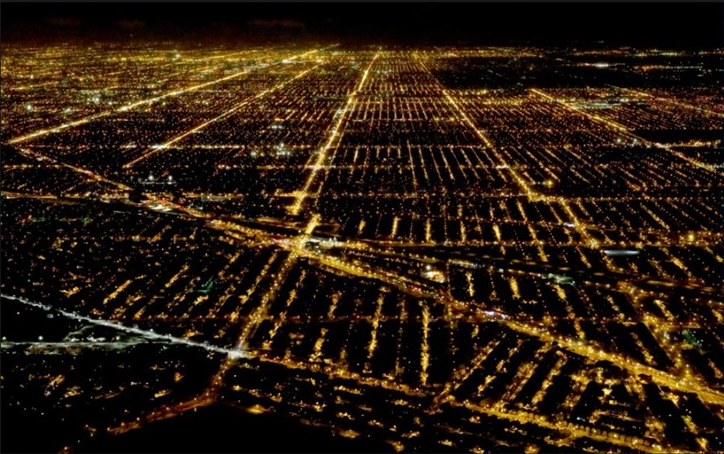
\includegraphics[scale=0.3]{Figures/title1.png}
        \label{ComplexSystems}
        \end{figure}
    \column{0.5\textwidth}
        \begin{figure}
        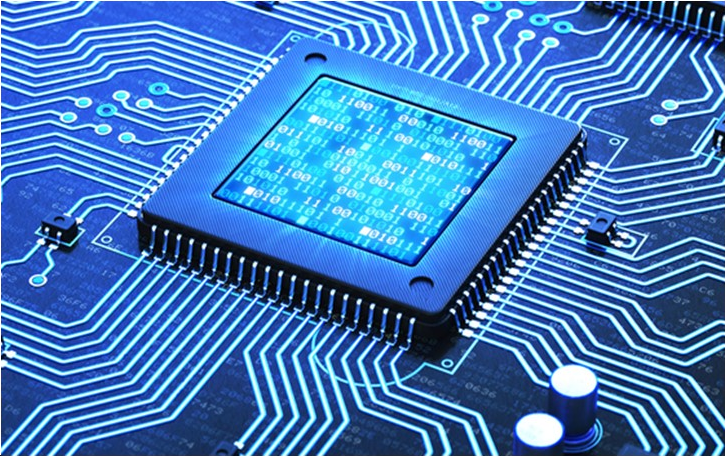
\includegraphics[scale=0.3]{Figures/title2.png}
        \label{ComplexAdaptiveSystem}
        \end{figure}
\end{columns}        
% ---------->	If you add author or date, reduce the following space <----------
		\vskip4em
		
	\end{frame}
	
	%Setting the background color to none
	\setbeamercolor{background canvas}{bg=}
	
% ---------->	Uncomment these lines for an automatically generated table of contents. <----------
	\begin{frame}{Outline}
	
	  \tiny\tableofcontents

	\end{frame}
	
	%----------------------------------Example section: Introduction----------------------------------
	\section{Background}
\begin{frame}
\frametitle{EV- before}


\begin{figure}
        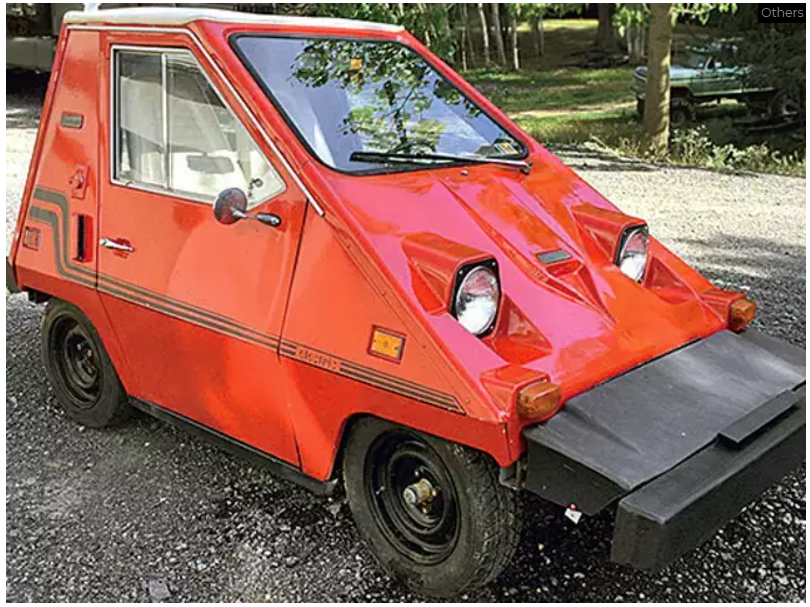
\includegraphics[scale=0.4]{Figures/EV80s.png}
        \caption{[ economictimes.indiatimes.com]}
        \end{figure}
\end{frame}
%%%%%%%%%%%%%%%%%%%%%%%%%%%%%%%%%
%%%%%%%%%%%%%%%%%%%%%%%%%%%%%%%%%%%
%%%%%%%%%%%%%%%%%%%%%%%%%%%%%%%%%%%%
%%%%%%%%%%%%%%%%%%%%%%%%%%%%%%%%%%%
%%%%%%%%%%%%%%%%%%%%%%%%%%%%%%%%%
\begin{frame}{EV- Now 379-mile range 610 km}
\begin{figure}
        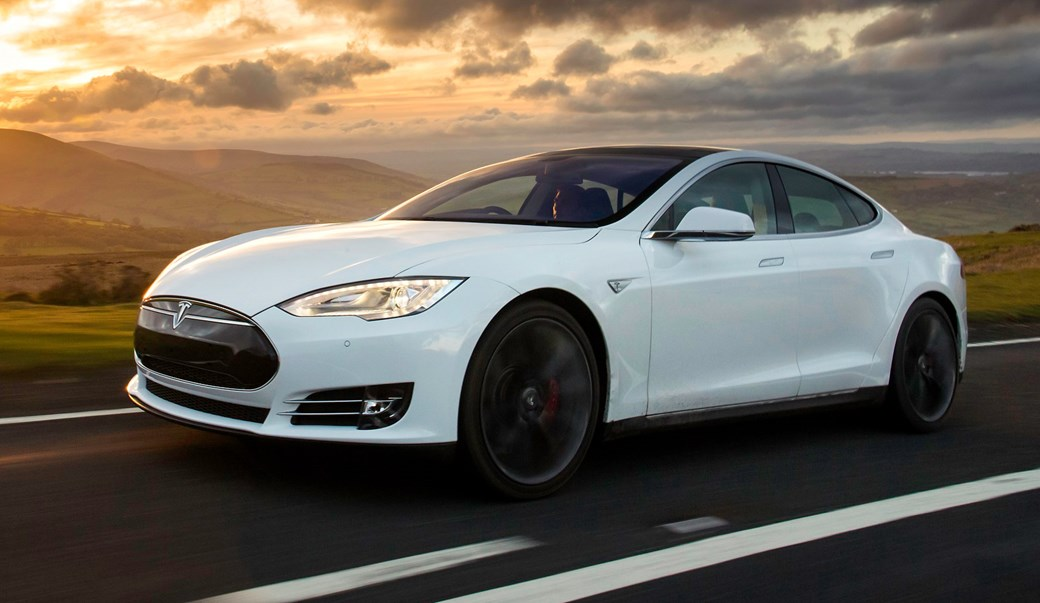
\includegraphics[scale=0.3]{Figures/EV2020.jpg}
        \caption{ [
 www.carmagazine.co.uk]}
        \end{figure}
\end{frame}

	%%%%%%%%%%%%%%%%%%%%%%%%%%%%%%%%%
%%%%%%%%%%%%%%%%%%%%%%%%%%%%%%%%%%%
%%%%%%%%%%%%%%%%%%%%%%%%%%%%%%%%%%%%
%%%%%%%%%%%%%%%%%%%%%%%%%%%%%%%%%%%
%%%%%%%%%%%%%%%%%%%%%%%%%%%%%%%%%
\begin{frame}{Statistics}
\only<1>{
\begin{block}{Market Share}
Market share of electric cars (BEV and PHEV) in Norway from 2009 to 2019
\end{block}
\center
        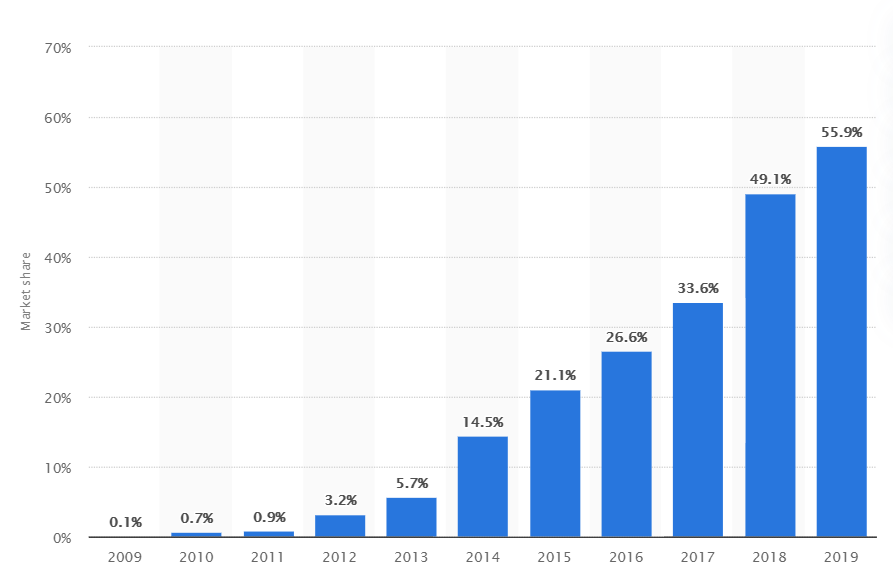
\includegraphics[scale=0.4]{Figures/marketShare.png}}
        \only<2>{
\begin{alertblock}{Penetration}
Around 9\% EV penetration in Norwegian transport sector. The Norwegian Parliament has decided on a national goal that all new cars sold by 2025 should be zero-emission (electric or hydrogen)\footnote{https://elbil.no/}.
\end{alertblock}}
\end{frame}

	%%%%%%%%%%%%%%%%%%%%%%%%%%%%%%%%%
%%%%%%%%%%%%%%%%%%%%%%%%%%%%%%%%%%%
%%%%%%%%%%%%%%%%%%%%%%%%%%%%%%%%%%%%
%%%%%%%%%%%%%%%%%%%%%%%%%%%%%%%%%%%
%%%%%%%%%%%%%%%%%%%%%%%%%%%%%%%%%
\begin{frame}{Is there any challenge?}
\only<1>{
\begin{figure}
        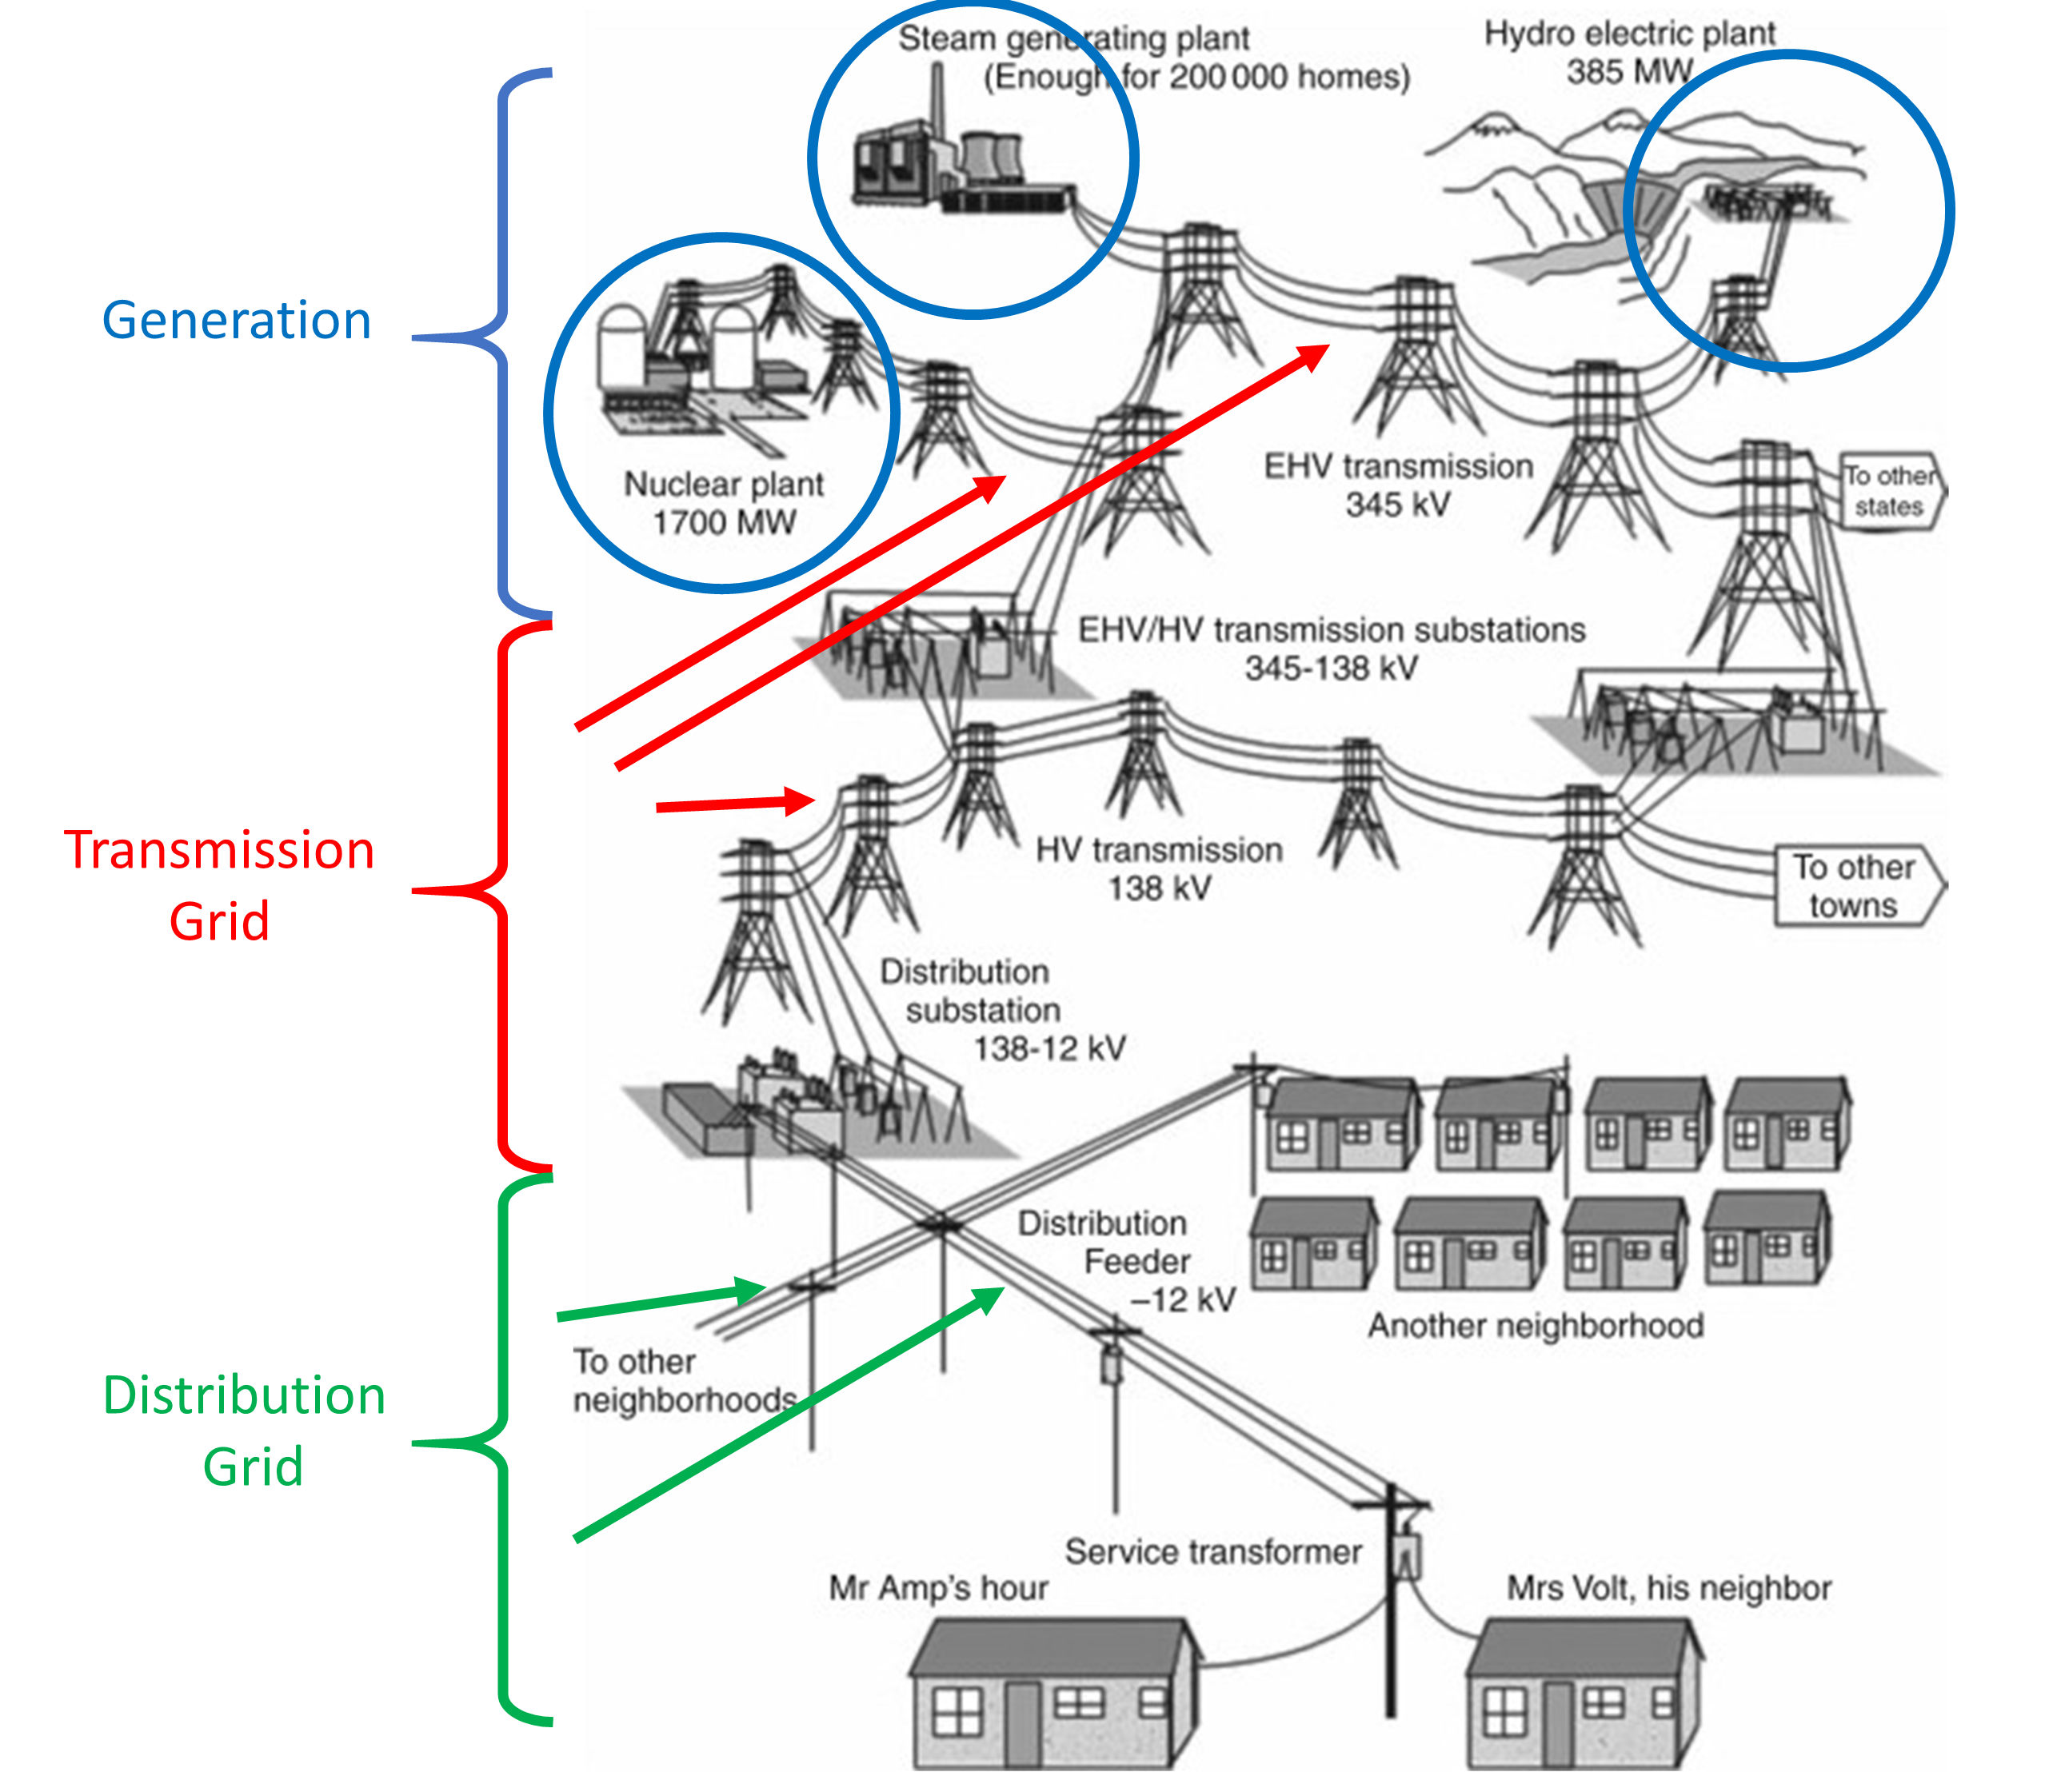
\includegraphics[scale=0.12]{Figures/PF.png}
        \caption{\tiny Source\footnote{\tiny https://www.sciencedirect.com/science/article/pii/B9781845697846500019
}}
\end{figure}}
\only<2>{\center 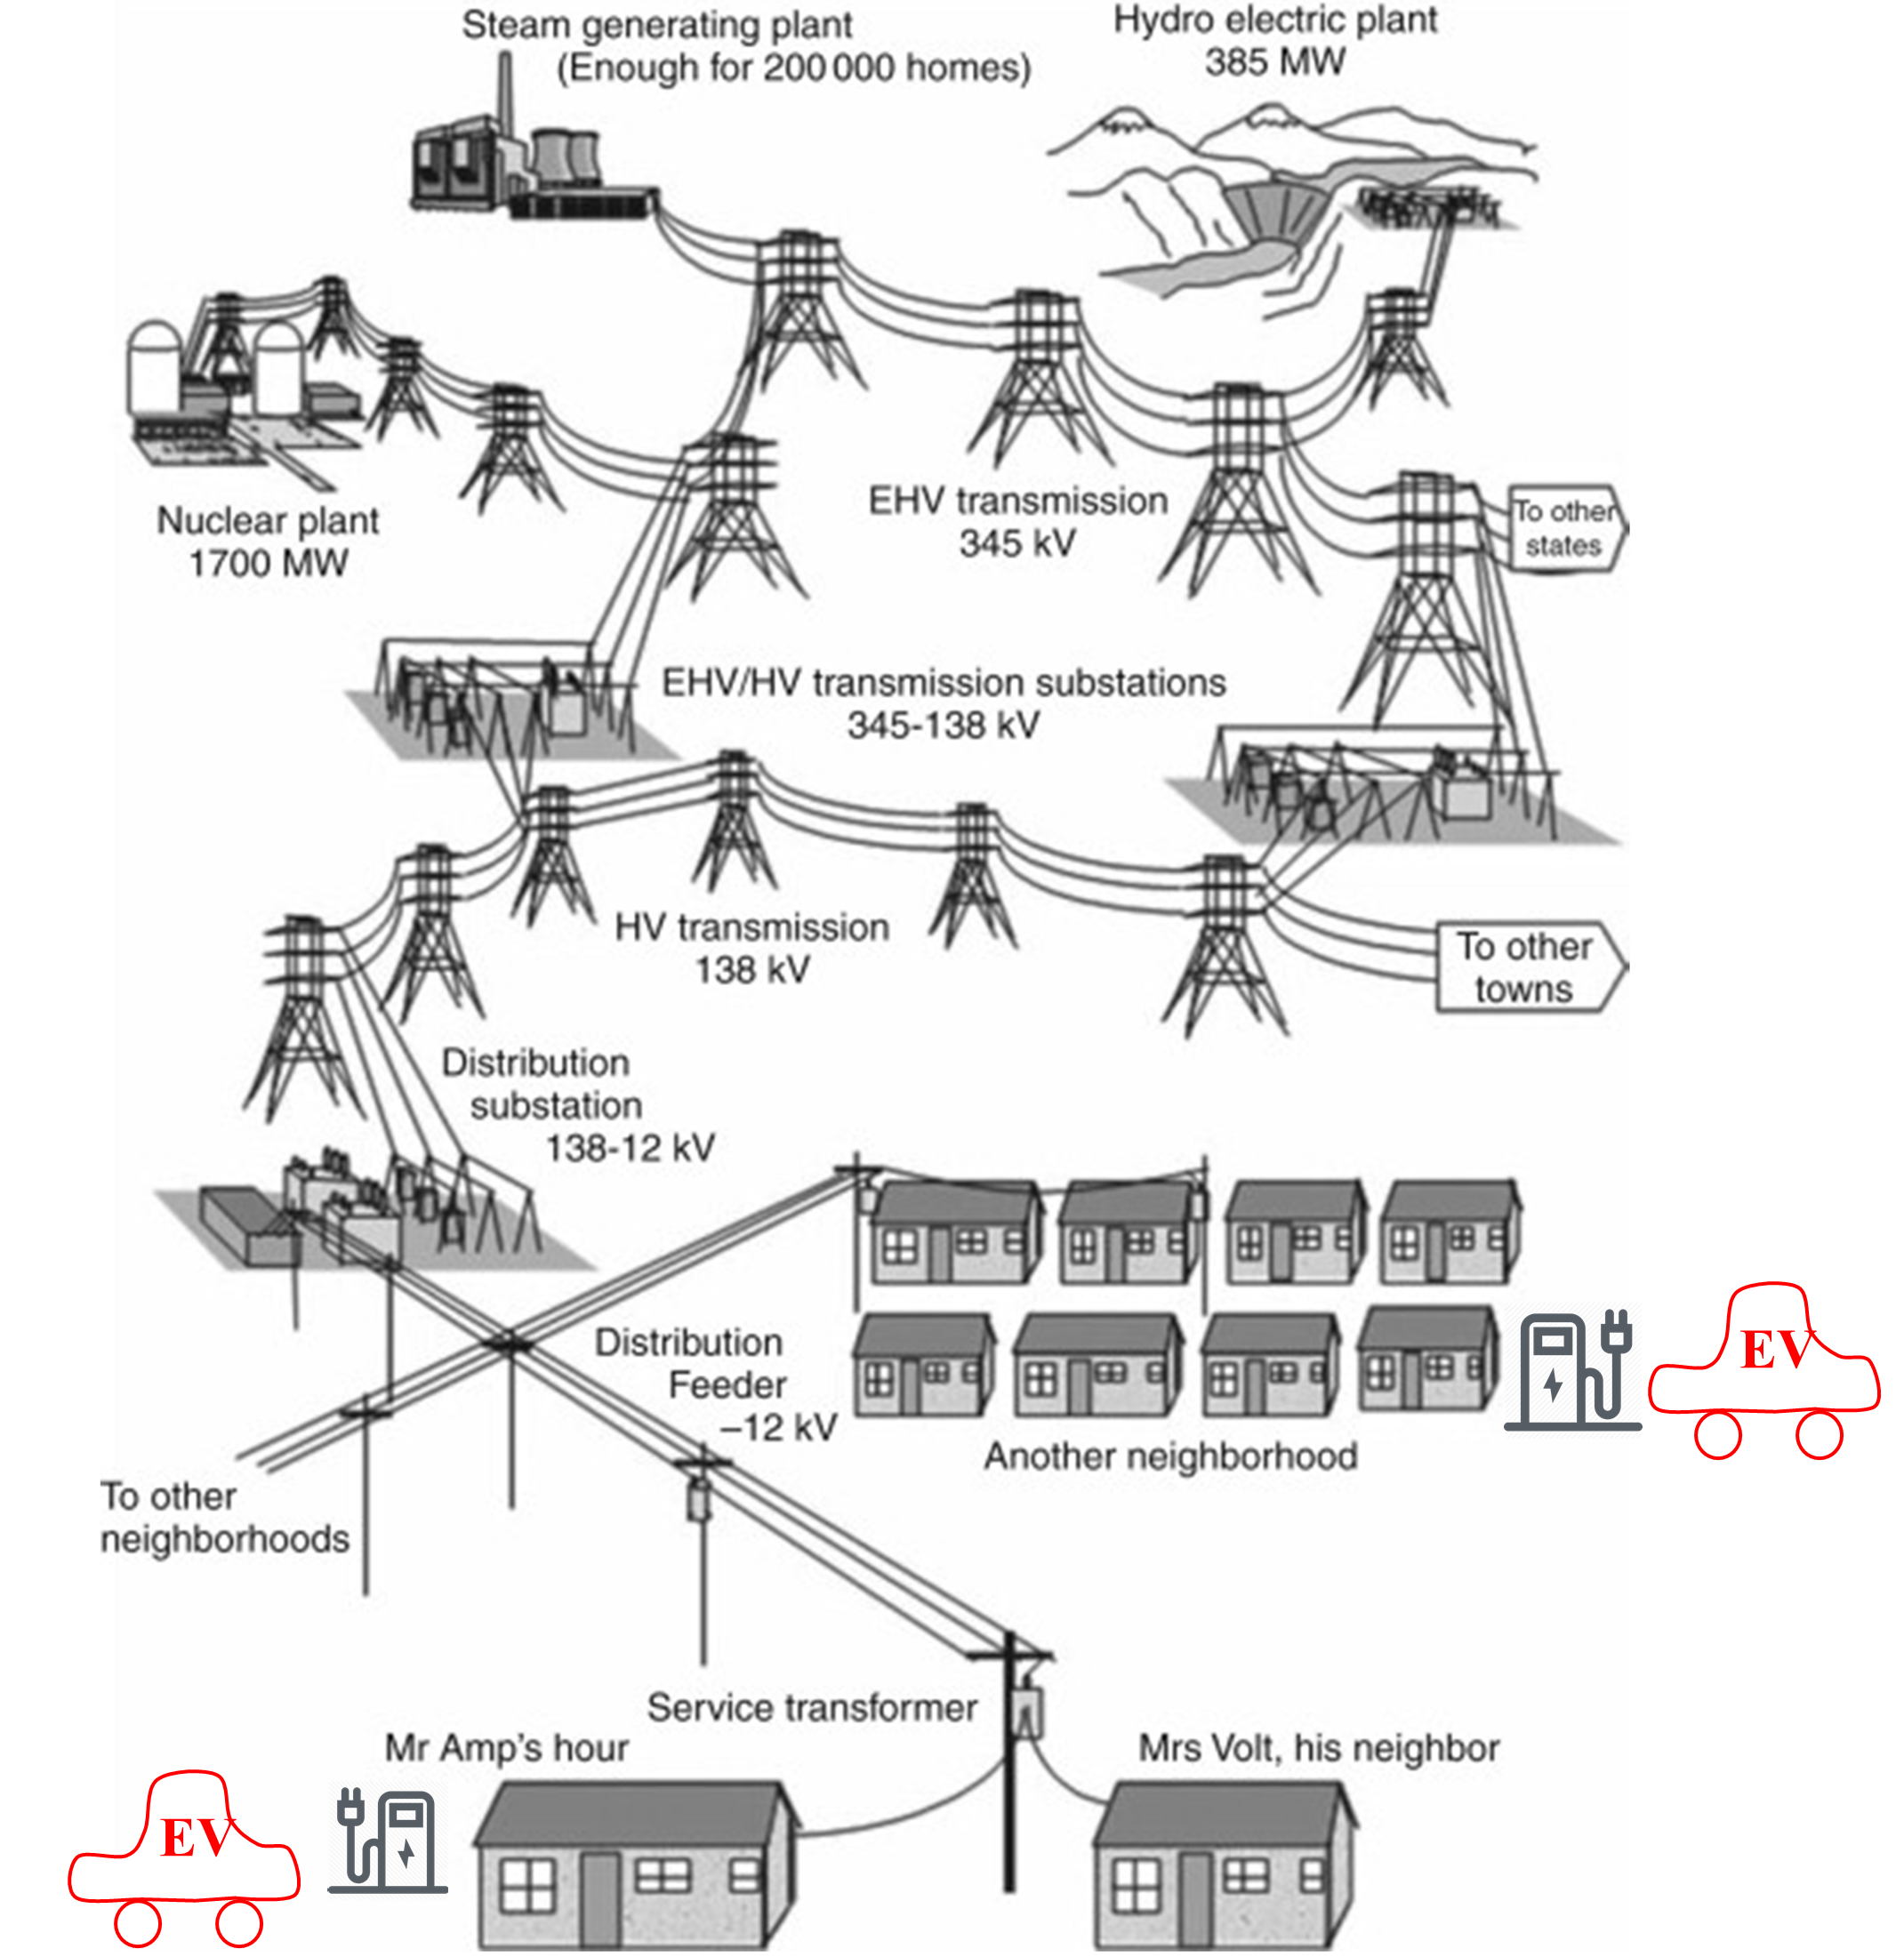
\includegraphics[scale=0.12]{Figures/EVchalendge1.png}}
\only<3>{\center 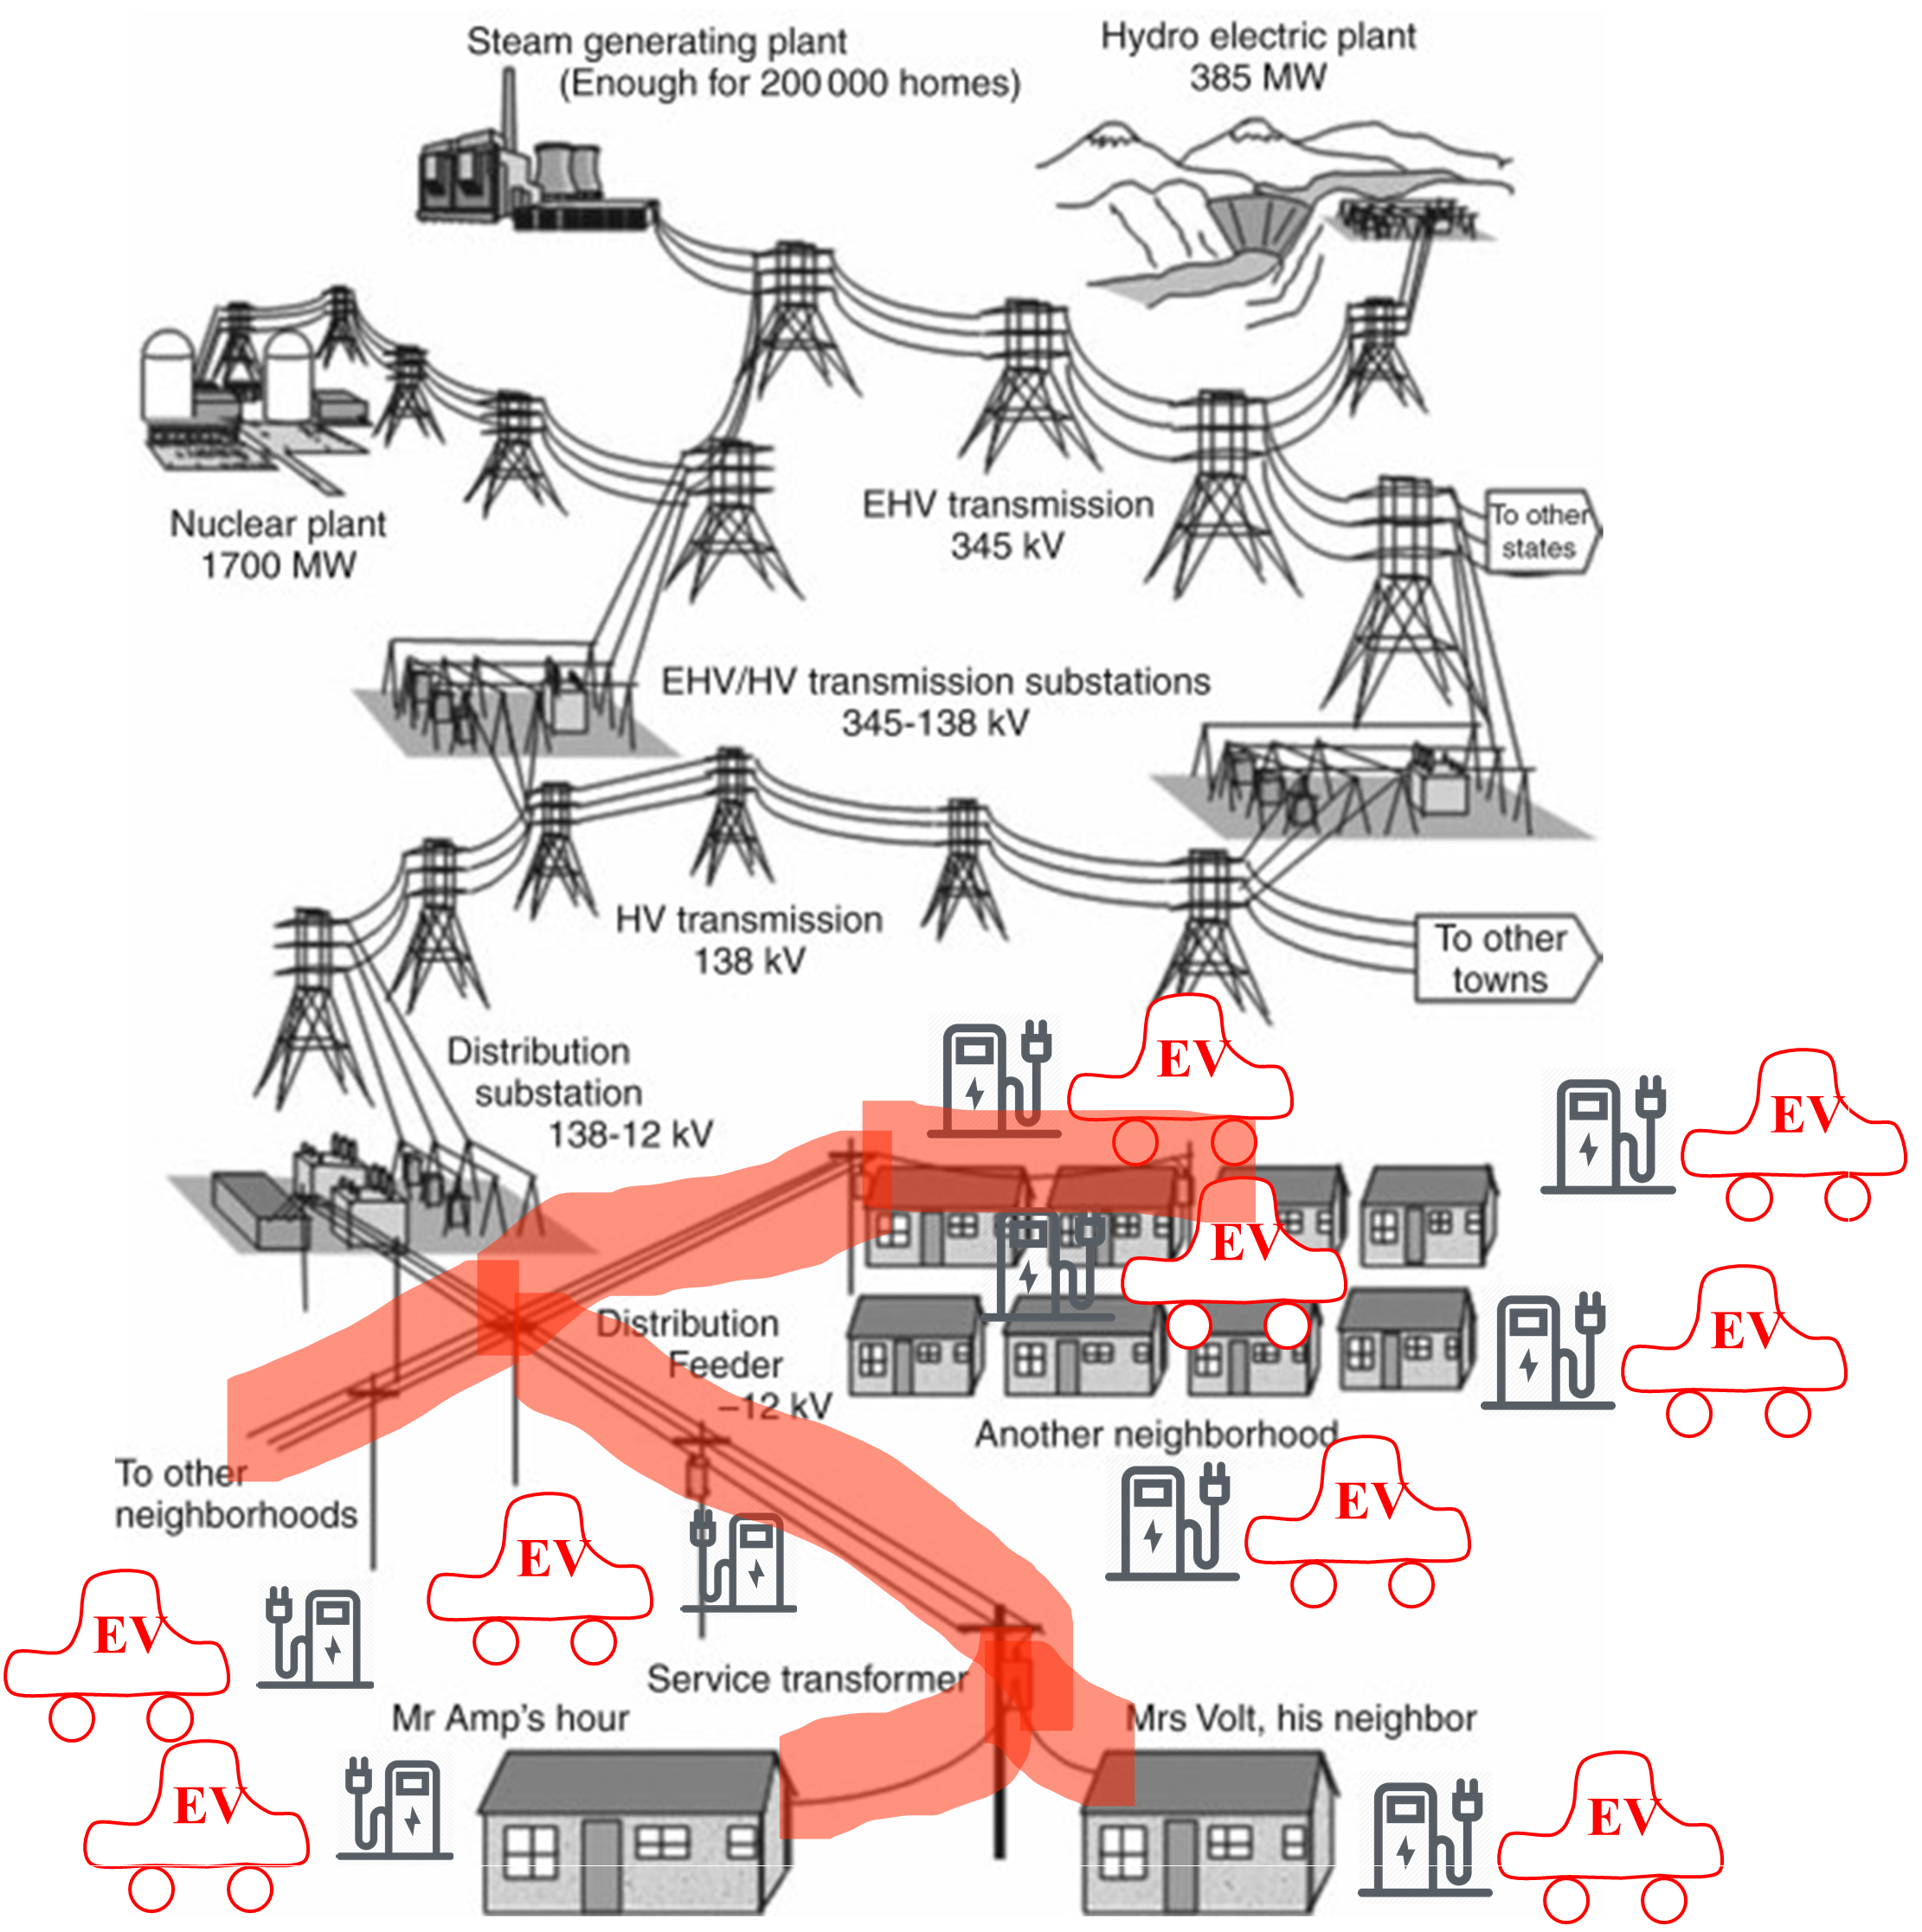
\includegraphics[scale=0.12]{Figures/EVchalendge2.png}}
\end{frame}

%%%%%%%%%%%%%%%%%%%%%%%%%%%%%%%%%
%%%%%%%%%%%%%%%%%%%%%%%%%%%%%%%%%%%
%%%%%%%%%%%%%%%%%%%%%%%%%%%%%%%%%%%%
%%%%%%%%%%%%%%%%%%%%%%%%%%%%%%%%%%%
%%%%%%%%%%%%%%%%%%%%%%%%%%%%%%%%%
\subsection{Challenge}

\begin{frame}{Challenge}
 \begin{alertblock}{}
 Distribution Grid will be under heavy stress in a near future!
 \end{alertblock}
 \begin{columns}
    \column{0.6\textwidth} 
 
    {\srcsize
\begin{table}[htbp!]
\begin{center}
\begin{tabular}{c c c c c} 
\hline 
\multicolumn{1}{c } {Scenario}&\begin{tabular}[c]{@{}c@{}}Number\\ of EV\\ per\\household \end{tabular} &\begin{tabular}[c]{@{}c@{}}Charging\\ Power (kW) \end{tabular} & \begin{tabular}[c]{@{}c@{}}Simultaneous\\ charge \end{tabular}& \begin{tabular}[c]{@{}c@{}}Additional\\ power\\ per house\\in max \\load (kW) \end{tabular} \\  
\hline\hline \rowcolor{Gray}
1 & 0.5 &5.1 &30\%&1\\
\hline
2 & 0.75 &6.0 &50\%&2\\
\hline \rowcolor{Gray}
3 & 1 &7.1 &70\%&5\\
\hline\hline
\end{tabular}
\end{center}
\end{table}}
\column{0.4\textwidth}
    {\srcsize
\begin{figure}
        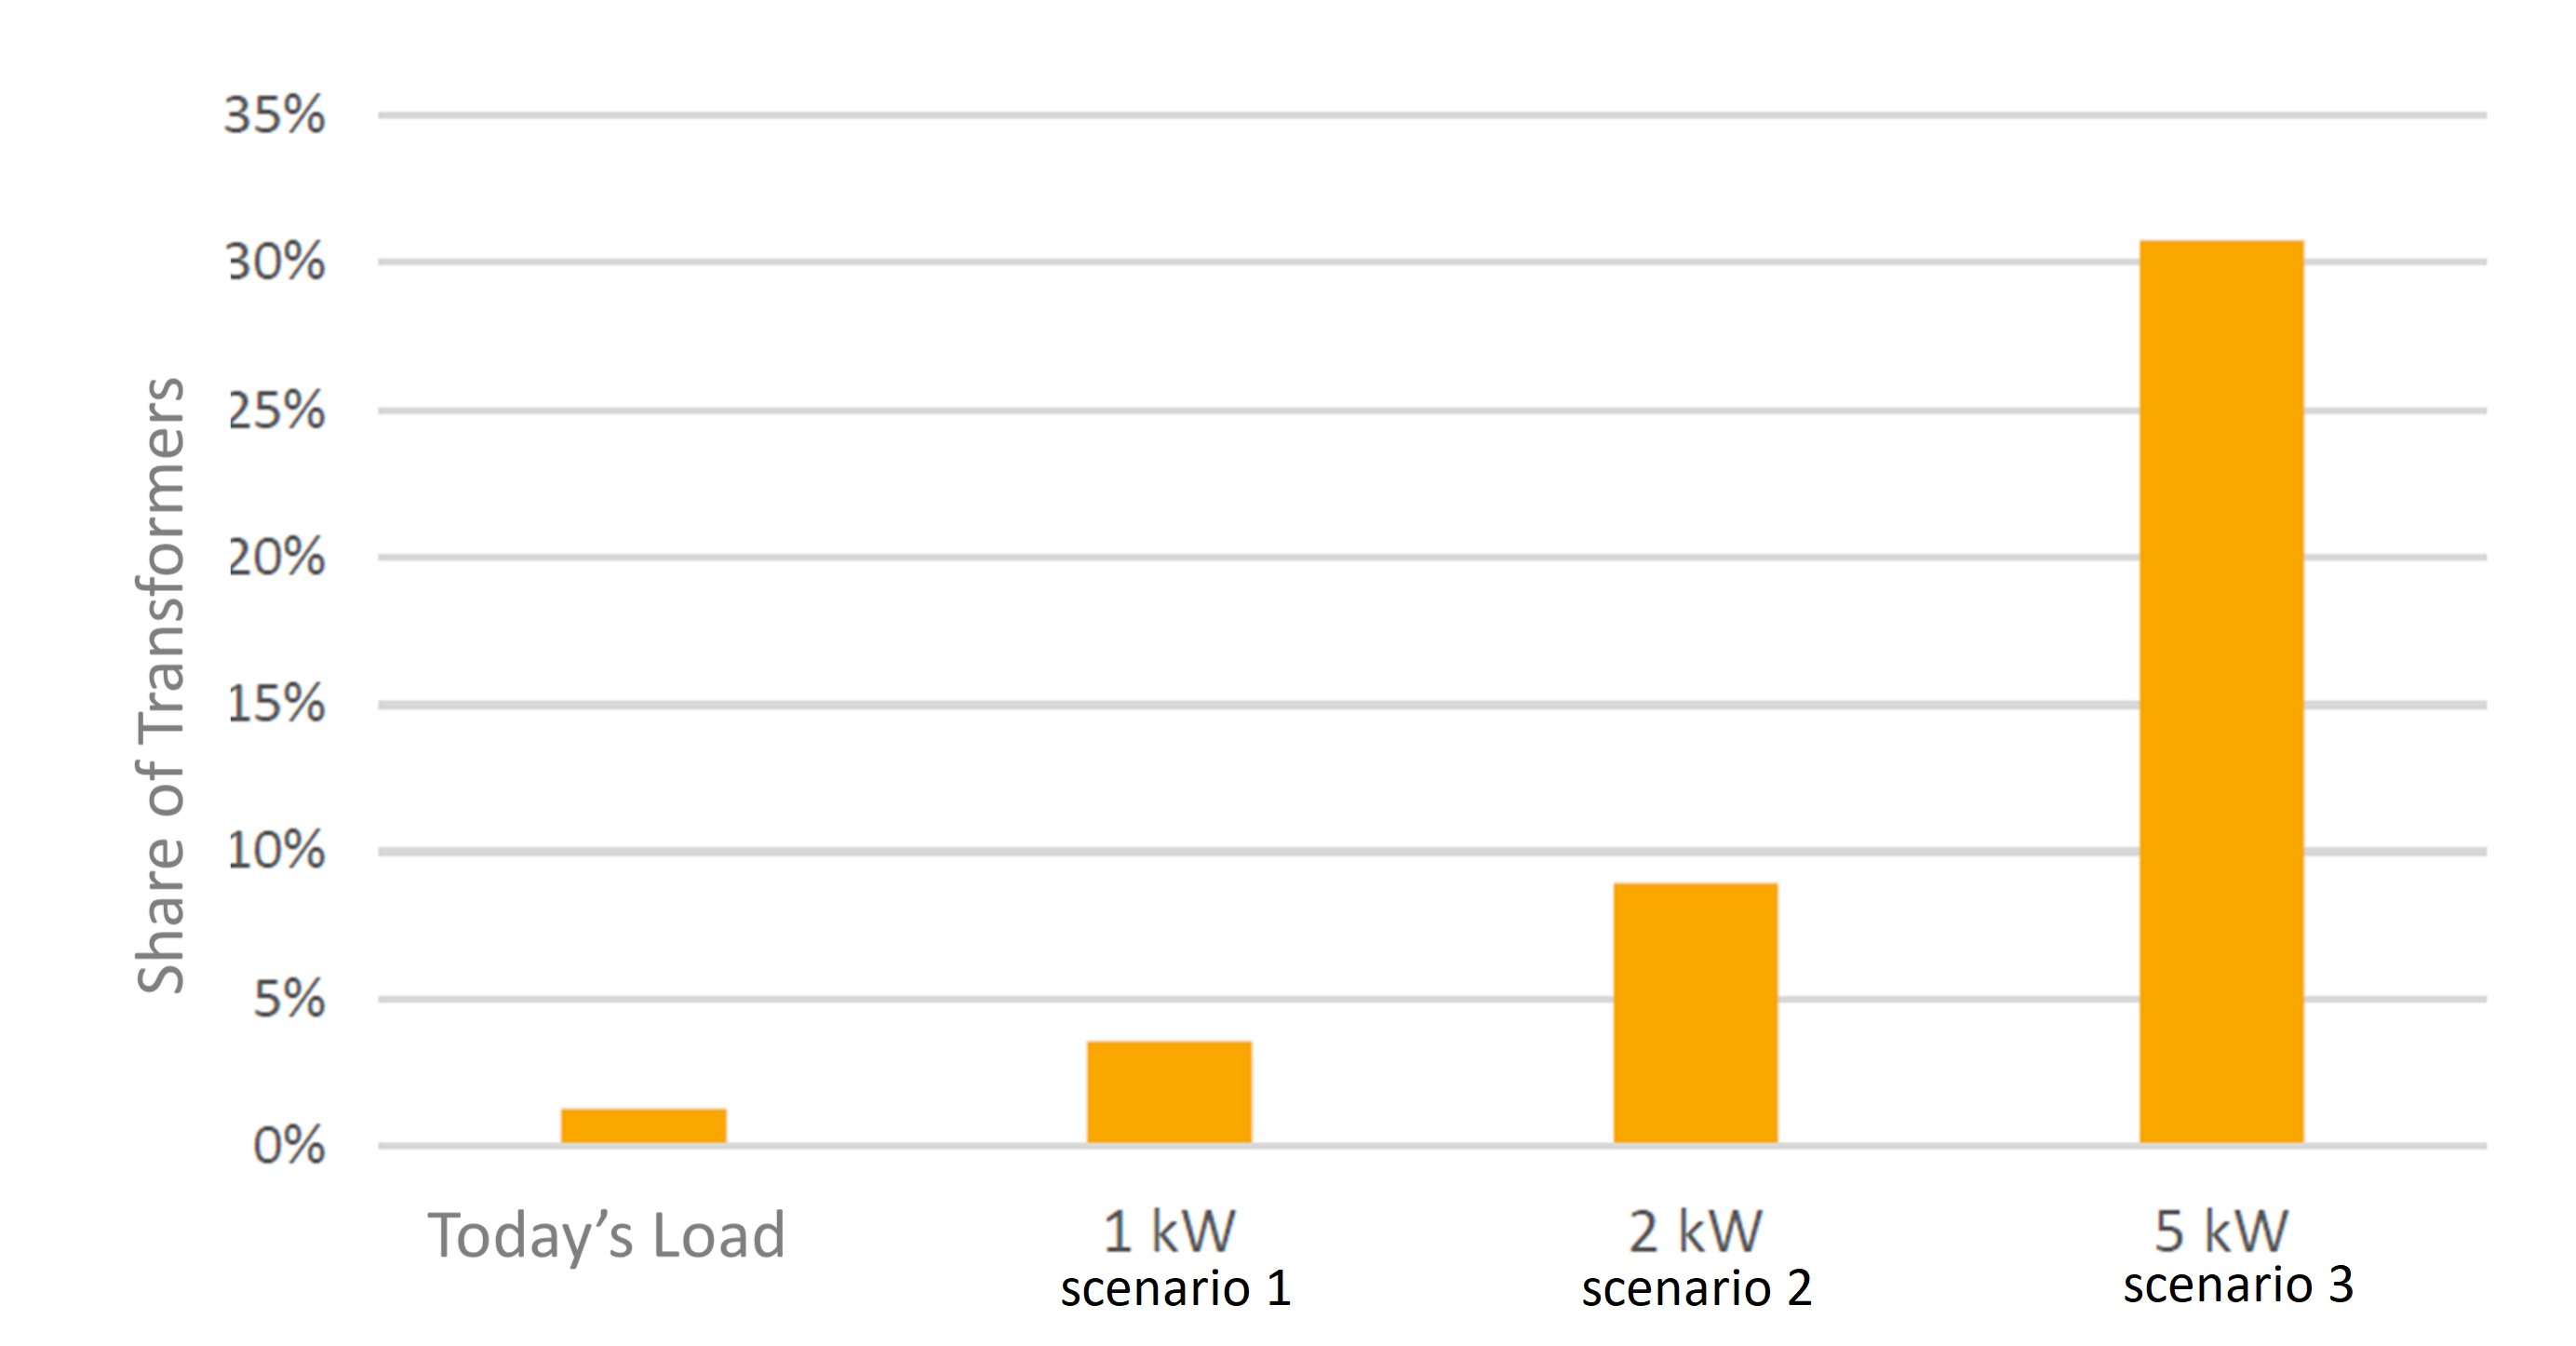
\includegraphics[scale=0.1]{Figures/TransOverLoad.png}
        \caption{\tiny The Norwegian Water Resources and Energy Directorate (NVE) Report  [Skotland, C. et al, "Hva betyr elbiler for strømnettet." (2016)]}
\end{figure}}
\end{columns}
\end{frame}
	%%%%%%%%%%%%%%%%%%%%%%%%%%%%%%%%%
%%%%%%%%%%%%%%%%%%%%%%%%%%%%%%%%%%%
%%%%%%%%%%%%%%%%%%%%%%%%%%%%%%%%%%%%
%%%%%%%%%%%%%%%%%%%%%%%%%%%%%%%%%%%
%%%%%%%%%%%%%%%%%%%%%%%%%%%%%%%%%

\begin{frame}{\small Dumb (Uncoordinated) VS Smart (Coordinated) Charging}
\begin{enumerate}[I.]
\item<1-> Dumb Charging
\begin{enumerate}
\item<2-> Anytime connects, it gets charged
\item<3-> No control on maximum power capacity usage
\end{enumerate}
\item<4-> Smart Charging
\begin{enumerate}
\item<5-> From user perspective:
\begin{itemize}
\item<6-> \textcolor{blue}{\textbf{>}} Sensitive to price? \only<6>{ 
        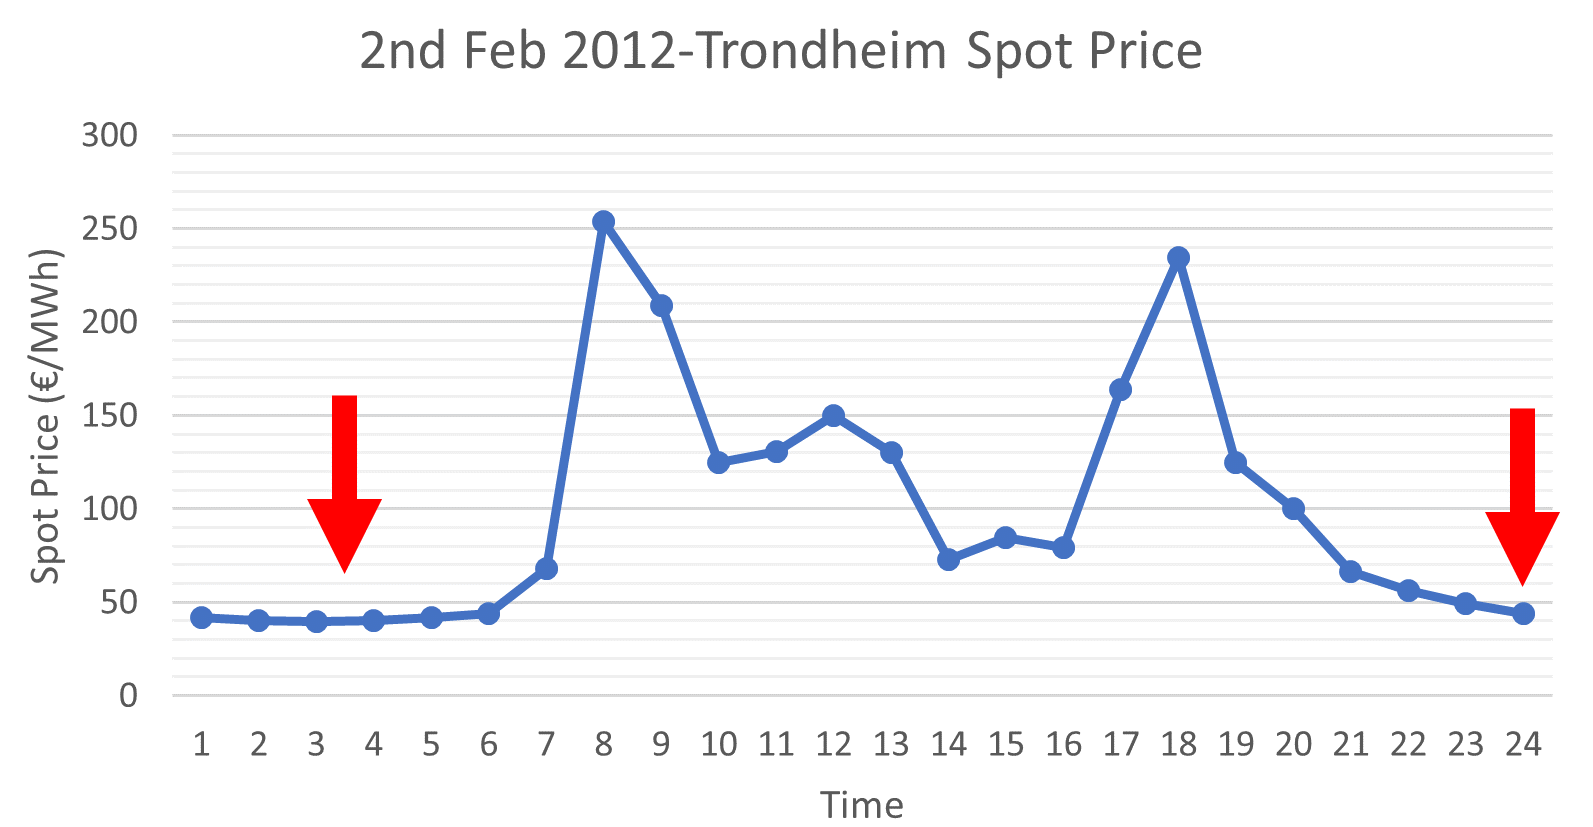
\includegraphics[scale=0.2]{Figures/SpotPrice.png}}
        
\item<7-> \visible<7-> {\textcolor{blue}{\textbf{>}} Sensitive to battery degradation?}
\end{itemize}
\item<8-> \visible<8-> {From distributor perspective:}
\begin{itemize}
\item<9-> \visible<9-> {\textcolor{blue}{\textbf{>}} Reliability of the distribution system?}
\item<10-> \visible<10-> {\textcolor{blue}{\textbf{>}} Cost of Investments?}
\item<11-> \visible<11-> {\textcolor{blue}{\textbf{>}} Cost of Operations?}
\item<12-> \visible<12-> {\textcolor{blue}{\textbf{>}} Socio-Economic Cost?}
\end{itemize}
\end{enumerate}
\end{enumerate}
\end{frame}




%%%%%%%%%%%%%%%%%%%%%%%%%%%%%%%%%
%%%%%%%%%%%%%%%%%%%%%%%%%%%%%%%%%%%
%%%%%%%%%%%%%%%%%%%%%%%%%%%%%%%%%%%%
%%%%%%%%%%%%%%%%%%%%%%%%%%%%%%%%%%%
%%%%%%%%%%%%%%%%%%%%%%%%%%%%%%%%%




	\section{Background}
	\subsection{Motivation}
	\begin{frame}{Motivation}
		\begin{enumerate}
  			\item<1-> \vskip -1cm Sustainability: {\footnotesize Need tools for analysing operating conditions resulting from renewables, EV, storage and flexible demand.}
  			\only<1>{\begin{backgroundblock}{40mm}{30mm}

\includegraphics[width=100mm]{Figures/pageMotive.png}
\end{backgroundblock}}
			\item<2-> Economics: {\footnotesize Norway electric industry revenues of 61.6 billion NOK in 2018\footnote{\label{note1} \tiny https://www.nve.no/energy-market-and-regulation/retail-market/electricity-disclosure-2018/}. 1\% savings worth 615 million NOK (estimated using \textsuperscript{\ref{note1}} \textsuperscript{and} \footnote{\tiny{https://www.nordpoolgroup.com/Market-data1/Dayahead/Volumes/NO/Hourly/?view=table}})} 


			\item<3-> Reliability: {\footnotesize Annual cost of power interruptions to Norway economy is 1600 MNOK/year (estimated using \footnote{\tiny http://publikasjoner.nve.no/rapport/2018/rapport2018\_74.pdf} \textsuperscript{and} \footnote{\tiny Samdal, K., Kjolle, G. H., Singh, B., \& Kvitastein, O. (2006, June). Interruption costs and consumer valuation of reliability of service in a liberalised power market. In 2006 International Conference on Probabilistic Methods Applied to Power Systems (pp. 1-7). IEEE.})   }
			

    
	\end{enumerate}
		\end{frame}	
	%%%%%%%%%%%%%%%%%%%%%%%%%%%%%%%%%
%%%%%%%%%%%%%%%%%%%%%%%%%%%%%%%%%%%
%%%%%%%%%%%%%%%%%%%%%%%%%%%%%%%%%%%%
%%%%%%%%%%%%%%%%%%%%%%%%%%%%%%%%%%%
%%%%%%%%%%%%%%%%%%%%%%%%%%%%%%%%%
	\subsection{Research Questions}
		\begin{frame}{Research Questions}
\begin{enumerate}[label=\textbf{RQ {\arabic*}.},ref=RQ {\arabic*}.]
\item<1-> \label{int:RQ1} With only ``passive charging'', the deployment of EVs will be limited by grid constraints. Can ``smart-charging'' overcome this problem?
\item<2-> \label{int:RQ2} How many additional EVs can be served by fast-charging points with a ``smart-charging'' regime compared to ``passive charging''? 
\begin{enumerate}[label=\textbf{C {\arabic*}.},ref=C {\arabic*}.]
\item<3-> \label{int:con1}  Without any reinforcements of the grid. 
\item<4-> \label{int:con2} Without any reduction in driving range.
\end{enumerate}
\item<5-> \label{int:RQ3} How much grid reinforcements is needed with smart vs passive-charging to fulfill increasing targets for an EV fleet as a replacement for gasoline and diesel cars?
\item<6-> \label{int:RQ4} Could integration of PV mitigate the impact of increasing EV penetration on the distribution grid?
\end{enumerate}
\end{frame}	
%%%%%%%%%%%%%%%%%%%%%%%%%%%%%%%%%
%%%%%%%%%%%%%%%%%%%%%%%%%%%%%%%%%%%
%%%%%%%%%%%%%%%%%%%%%%%%%%%%%%%%%%%%
%%%%%%%%%%%%%%%%%%%%%%%%%%%%%%%%%%%
%%%%%%%%%%%%%%%%%%%%%%%%%%%%%%%%%
\subsection{Tasks}
		\begin{frame}{Tasks}
\begin{enumerate}[label=\textbf{Task {\arabic*}.},ref=Task {\arabic*}.]
\item<1-> \label{int:task1} Develop a smart-charging algorithm/scheme with the objective to compare and analyse how many additional EVs can be served by a smart-charging method.
\item<2-> \label{int:task2} Develop a simulator for the combined power-and-transport system.
\item<3-> \label{int:task3} Simulate the combined system with an increasing number of charging points (and cars), and measure the ``saturation point'' with respect to the requirements in \ref{int:RQ2}.
\item<4-> \label{int:task4} Develop a power flow solver that takes into account the operational grid constraints, grid losses and also local generations.
\item<5-> \label{int:task5} Investigate the impact of growing penetration of EVs and PVs together in the distribution grid.
\end{enumerate}
\end{frame}	
%%%%%%%%%%%%%%%%%%%%%%%%%%%%%%%%%
%%%%%%%%%%%%%%%%%%%%%%%%%%%%%%%%%%%
%%%%%%%%%%%%%%%%%%%%%%%%%%%%%%%%%%%%
%%%%%%%%%%%%%%%%%%%%%%%%%%%%%%%%%%%
%%%%%%%%%%%%%%%%%%%%%%%%%%%%%%%%%
\section{Publications}
\begin{frame}{Relevant to Thesis}
\begin{enumerate}[I.]
{\tiny \vskip -0.2cm
\begin{alertblock}{Under Review}
\item S. Zaferanlouei, H. Farahmand, V. Vadlamudi, and M. Korpås, “BATTPOWER Toolbox: Memory Efficient and High-Performance MultiPeriod AC Optimal Power Flow Solver—Part I: Mathematical Concepts,” submitted for review, IEEE transaction on Power Systems, 2020.
\item S. Zaferanlouei, H. Farahmand, V. Vadlamudi, and M. Korpås, “BATTPOWER Toolbox: Memory Efficient and High-Performance MultiPeriod AC Optimal Power Flow Solver—Part II: Case Study,” submitted for review, IEEE transaction on Power Systems, 2020.
\item  S. Zaferanlouei, V. Lakshmanan, S. Bjarghov, H. Farahmand and M. Korpås, “BATTPOWER Application: Large Scale Integration of EVs in a Local Distribution Grid—Norwegian Case Study,” submitted for review, Electric Power Systems Research, 2020.
\end{alertblock} \vskip -0.2cm
\begin{block}{Publised}
\item S. Zaferanlouei, M. Korpås, J. Aghaei, H. Farahmand and N. Hashemipour, “Computational Efficiency Assessment of Multi-Period AC Optimal Power Flow including Energy Storage Systems,” in 2018 International Conference on Smart Energy Systems and Technologies (SEST), Sep. 2018, pp. 1– 6. DOI: \href{10.1109/SEST.2018.8495683}{10.1109/SEST.2018.8495683}.
\item S. Zaferanlouei, M. Korpås, H. Farahmand and V. V. Vadlamudi, “Integration of PEV and PV in Norway Using Multi-Period ACOPF—Case study,” in 2017 IEEE Manchester PowerTech, ISSN: null, Jun. 2017, pp. 1–6. DOI: \href{10.1109/PTC.2017.7981042}{10.1109/PTC.2017.7981042}.
\item S. Zaferanlouei, I. Ranaweera, M. Korpås and H. Farahmand, “Optimal Scheduling of Plug-in Electric Vehicles in Distribution Systems Including PV, Wind and Hydropower Generation, eng. Energynautics GMBH, 2016,” ISBN: 978-3-9816549-3-6.
\item S. Flinstad Harbo, S. Zaferanlouei and M. Korpås, “Agent Based Modelling and Simulation of Plug-In Electric Vehicles Adoption in Norway,” in 2018 Power Systems Computation Conference (PSCC), Jun. 2018, pp. 1– 7. DOI: \href{10.23919/PSCC.2018.8442514}{10.23919/PSCC.2018.8442514}.
\item M. Lillebo, S. Zaferanlouei, A. Zecchino and H. Farahmand, “Impact of large-scale EV integration and fast chargers in a Norwegian LV grid,” The Journal of Engineering, vol. 2019, no. 18, pp. 5104–5108, 2019, ISSN: 2051-3305. DOI: \href{10.1049/joe.2018.9318}{10.1049/joe.2018.9318}.
\item S. Bjarghov, M. Korpås and S. Zaferanlouei, “Value comparison of EV and house batteries at end-user level under different grid tariffs,” in 2018 IEEE International Energy Conference (ENERGYCON), Jun. 2018, pp. 1–6. DOI: \href{10.1109/ENERGYCON.2018.8398742}{10.1109/ENERGYCON.2018.8398742}.
\end{block}}
\end{enumerate}
\end{frame}
%%%%%%%%%%%%%%%%%%%%%%%%%%%%%%%%%
%%%%%%%%%%%%%%%%%%%%%%%%%%%%%%%%%%%
%%%%%%%%%%%%%%%%%%%%%%%%%%%%%%%%%%%%
%%%%%%%%%%%%%%%%%%%%%%%%%%%%%%%%%%%
%%%%%%%%%%%%%%%%%%%%%%%%%%%%%%%%%
\begin{frame}{Other Publications}
\begin{enumerate}[I.]
{\footnotesize
\begin{alertblock}{under review}
\item G. Sæther, P. Crespo del Granadob, S. Zaferanlouei, “Peer-to-Peer electricity trading in an Industrial site:Value of buildings flexibility on peak load reduction,” Submitted on Energy and Buildings, Elsevier 2020.
\end{alertblock}
\begin{block}{Published}
\item F. Berglund, S. Zaferanlouei, M. Korpås and K. Uhlen, (2019). “Optimal Operation of Battery Storage for a Subscribed Capacity-Based Power Tariff Prosumer—A Norwegian Case Study,” Energies, 12(23), 4450.
\end{block}
}

\end{enumerate}
\end{frame}
%%%%%%%%%%%%%%%%%%%%%%%%%%%%%%%%%
%%%%%%%%%%%%%%%%%%%%%%%%%%%%%%%%%%%
%%%%%%%%%%%%%%%%%%%%%%%%%%%%%%%%%%%%
%%%%%%%%%%%%%%%%%%%%%%%%%%%%%%%%%%%
%%%%%%%%%%%%%%%%%%%%%%%%%%%%%%%%%


%%%%%%%%%%%%%%%%%%%%%%%%%%%%%%%%%
%%%%%%%%%%%%%%%%%%%%%%%%%%%%%%%%%%%
%%%%%%%%%%%%%%%%%%%%%%%%%%%%%%%%%%%%
%%%%%%%%%%%%%%%%%%%%%%%%%%%%%%%%%%%
%%%%%%%%%%%%%%%%%%%%%%%%%%%%%%%%%
\section{Power Flow}
\begin{frame}{Power Flow Equations}
\vskip -0.2cm

\begin{block}{Source of Non-linearity}
\textcolor{red}{Nonlinear relationship} between the voltage phasors and the power injections
\end{block}
\vskip -0.5cm
\begin{table}[htbp!]
\begin{tabular}{|r l| l|} 
\hline
\multicolumn{3}{|c|}{ 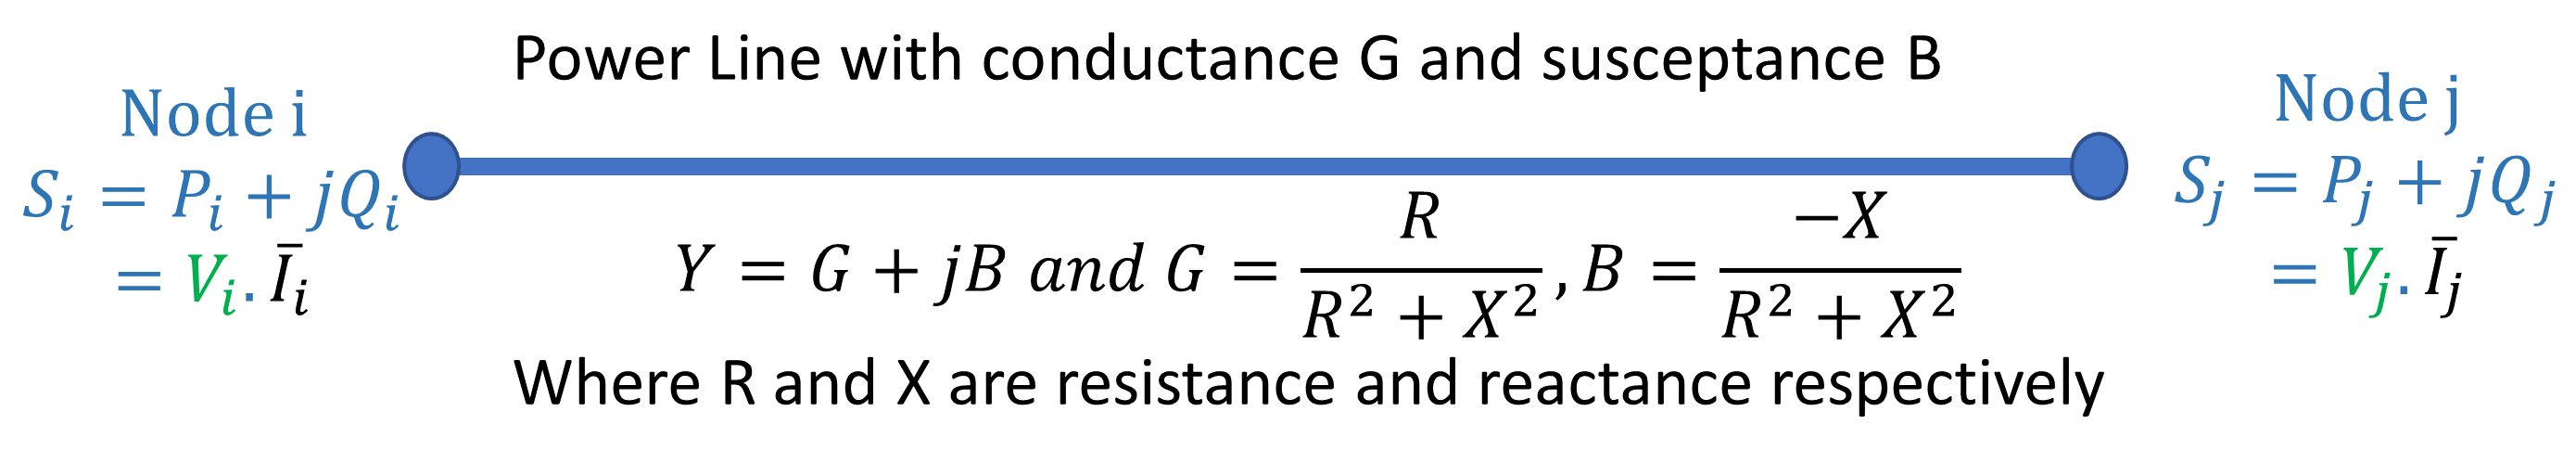
\includegraphics[scale=.15]{Figures/PowerFlow.png}}\\
\hline
 $\textcolor{blue}{P_i}+j\textcolor{blue}{Q_i} $&$= \textcolor{green}{V_i}.\overline{I}_i$& \\
 &$=\textcolor{green}{V_i}.(\mathbf{\overline{Y}}_i.\textcolor{green}{\overline{V}})$& $\mathbf{{Y}}$ \ admittance matrix\\
 &$=\textcolor{green}{V_i}. (\mathbf{G}_i-j\mathbf{B}_i)\textcolor{green}{\overline{V}}$& $\mathbf{{G}}$ and $\mathbf{{B}}$ \ conductance and susceptance matrices\\
 $\textcolor{green}{|V_i|^2}$&$=\textcolor{green}{V_i}.\textcolor{green}{\overline{V}_i}$&$\mathbf{{Y}}=\mathbf{G}+j\mathbf{B}$\\
 \multicolumn{2}{|c|}{"Power Flow Equations"}&\\
 \multicolumn{2}{|c|}{"Load Flow Equations"}&\\
 \hline
 \end{tabular}
\end{table}
\begin{itemize}[label={>}]
\item \textcolor{red}{Coupled quadratics} in complex voltage phasors
\end{itemize}
\end{frame}

%%%%%%%%%%%%%%%%%%%%%%%%%%%%%%%%%
%%%%%%%%%%%%%%%%%%%%%%%%%%%%%%%%%%%
%%%%%%%%%%%%%%%%%%%%%%%%%%%%%%%%%%%%
%%%%%%%%%%%%%%%%%%%%%%%%%%%%%%%%%%%
%%%%%%%%%%%%%%%%%%%%%%%%%%%%%%%%%
\begin{frame}{Power Flow Equations in Different Coordinates}

\onslide<1-2>{\scriptsize {The \textcolor{red}{bus injection} model
\begin{center}
\begin{tabular}{|c c|} 
\hline
\multicolumn{2}{|c|}{ 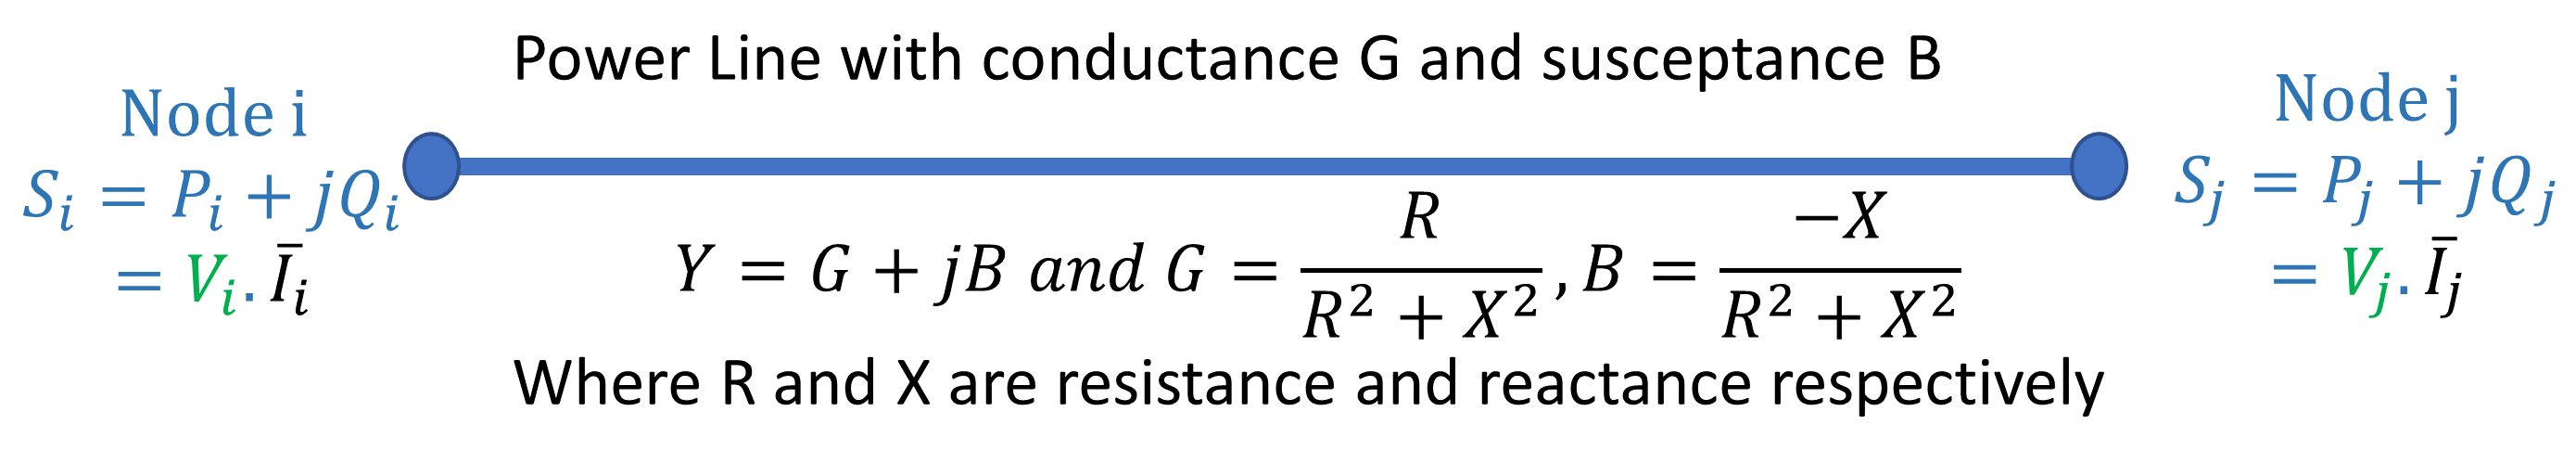
\includegraphics[scale=.15]{Figures/PowerFlow.png}}\\
\hline
 \multicolumn{1}{|c|}{Polar Voltage Coordinates}&$\textcolor {green}{V_i}=\textcolor {green}{\abs{V_i}}\angle \textcolor {green}{\theta_i}$\quad $\textcolor {green}{\theta_1}=0$\\  
\cline{1-1}
\multicolumn{2}{|c|}{$ 
 \textcolor {blue}{P_{i}} =\textcolor {green}{\abs{V_{i}}}\sum_{j=1}^{N} \textcolor {green}{\abs{V_{j}}} (\boldsymbol{G}_{ij} cos(\textcolor {green}{\theta{i}}-\textcolor {green}{\theta{j}})+\boldsymbol{B}_{ij}sin(\textcolor {green}{\theta{i}}-\textcolor {green}{\theta{j}}))$}\\

\multicolumn{2}{|c|}{$ \textcolor {blue}{Q_{i}} =\textcolor {green}{\abs{V_{i}}}\sum_{j=1}^{N}
 \textcolor {green}{\abs{V_{j}}} (\boldsymbol{G}_{ij} sin(\textcolor {green}{\theta{i}}-\textcolor {green}{\theta{j}})-\boldsymbol{B}_{ij}cos(\textcolor {green}{\theta{i}}-\textcolor {green}{\theta{j}}))$}\\
 \hline\hline
  \multicolumn{1}{|c|}{Rectangular Voltage Coordinates}&$\textcolor {green}{V_i}=\textcolor {green}{V_{di}}+j \textcolor {green}{V_{qi}}$\quad $\textcolor {green}{V_{q1}}=0$\\  
\cline{1-1}
\multicolumn{2}{|c|}{$ 
 \textcolor {blue}{P_{i}} =\textcolor {green}{V_{di}}(\boldsymbol{G}_{ij} \textcolor {green}{V_{dj}} -\boldsymbol{B}_{ij} \textcolor {green}{V_{qj}})
 +
 \textcolor {green}{V_{qi}}(\boldsymbol{B}_{ij} \textcolor {green}{V_{dj}} +\boldsymbol{G}_{ij} \textcolor {green}{V_{qj}})$}\\

\multicolumn{2}{|c|}{$ 
 \textcolor {blue}{Q_{i}} =-\textcolor {green}{V_{di}}(\boldsymbol{B}_{ij} \textcolor {green}{V_{dj}} +\boldsymbol{G}_{ij} \textcolor {green}{V_{qj}})
 +
 \textcolor {green}{V_{qi}}(\boldsymbol{G}_{ij} \textcolor {green}{V_{dj}} -\boldsymbol{B}_{ij} \textcolor {green}{V_{qj}})$}\\

$ \textcolor {green}{V_{di}}= Re (\textcolor {green}{V_i})$ \  $ \textcolor {green}{V_{qi}}= Im (\textcolor {green}{V_i})$& $N=$ number of Nodes\\
  \hline
\end{tabular}
\end{center}}}
\onslide<2-> {\scriptsize \begin{block}{Power Flow}
PF equations are a set of nonlinear algebraic equations which can be solved with Newton-Raphson, Gauss–Seidel, Fast-decoupled-load-flow method and etc.
\end{block}}

\end{frame}
%%%%%%%%%%%%%%%%%%%%%%%%%%%%%%%%%
%%%%%%%%%%%%%%%%%%%%%%%%%%%%%%%%%%%
%%%%%%%%%%%%%%%%%%%%%%%%%%%%%%%%%%%%
%%%%%%%%%%%%%%%%%%%%%%%%%%%%%%%%%%%
%%%%%%%%%%%%%%%%%%%%%%%%%%%%%%%%%
\subsection{Single Period ACOPF}
\begin{frame}{Single period ACOPF - problem formulation}
\begin{block}{Single Period AC Optimal Power Flow (ACOPF)}
We are controlling some variables in OPF to minimise system costs with respect to constraints. 
\end{block}
\begin{center}
\begin{tabular}{|l l|} 
\hline
Objective Function&$\min_{\mathbf{x}} f(\mathbf{x})$\\  
\rowcolor{Gray}
\begin{tabular}[l]{@{}l@{}}Equality Constraints\\ (Balance)\\ Power Flow \end{tabular}  &$\textrm{s.t. }  \mathbf{g}(\mathbf{x})= \begin{colorbmatrix}
   \mathbf{\widetilde{g}}(\mathbf{x})\\
   \mathbf{\overline{g}}(\mathbf{x})
\end{colorbmatrix}=0 \qquad \in   \mathbb{R}^{n_{gx} \times 1}$\\
  
\begin{tabular}[l]{@{}l@{}}Inequality constraints\\ (line and transformer)\\ Operational Constraints \end{tabular}  & $\mathbf{h}(\mathbf{x})=\begin{colorbmatrix}
   \mathbf{\widetilde{h}}(\mathbf{x})\\
   \mathbf{\overline{h}}(\mathbf{x})
\end{colorbmatrix}\leq 0 \qquad \in   \mathbb{R}^{n_{hx} \times 1} $\\
\rowcolor{Gray}
Vector of Variables&$ \mathbf{x}= \big[\boldsymbol{\Theta}\  \boldsymbol{\mathcal{V}} \  \boldsymbol{\mathcal{P}}^{\mathrm{g}} \ \boldsymbol{\mathcal{Q}}^{\mathrm{g}} \big]^\top
 \in \mathbb{R}^{n_{x}\times 1}$\\  
\hline
\end{tabular}
\end{center}


\end{frame}
%%%%%%%%%%%%%%%%%%%%%%%%%%%%%%%%%
%%%%%%%%%%%%%%%%%%%%%%%%%%%%%%%%%%%
%%%%%%%%%%%%%%%%%%%%%%%%%%%%%%%%%%%%
%%%%%%%%%%%%%%%%%%%%%%%%%%%%%%%%%%%
%%%%%%%%%%%%%%%%%%%%%%%%%%%%%%%%%
\subsection{Limitations of PF and single period OPF}
\begin{frame}
\onslide<1->
{\footnotesize
\begin{block}{Limitation of Power Flow}
\begin{tabular}{|l|} 
\hline
\rowcolor{Gray}
\qquad \tabitem PF is only a set of static equations which provides status of a system for time: $t=t_s$\\
\rowcolor{Gray} \qquad \tabitem It does not include  generation constraints and operational constraints\\
\hline
\end{tabular}
\end{block}
}

\onslide<2->
{\footnotesize
\begin{block}{
Limitation of Single Period AC Optimal Power Flow}

\begin{tabular}{|l|} 
\hline
\rowcolor{Gray} \qquad \tabitem OPF is an optimisation problem which optimises status of a system\\
\rowcolor{Gray}\ \ \qquad for a SINGLE time: $t=t_s$.\\
\rowcolor{Gray} \qquad \tabitem Although it includes the operational constraints for single time,\\
\rowcolor{Gray}\ \ \qquad it will not include operation of DERs and generators over a time horizon.\\
\rowcolor{Gray} \qquad \tabitem It is not capable of integrating storage devices and EVs. \\
\hline
\end{tabular}
}
\end{block}
\onslide<3->
\begin{alertblock}
{ Our suggested approach: multi-period ACOPF}
{ Solves the OPF problem over several time-steps at once useful formulation for systems with Energy Storage and Shiftable Loads (e.g. Evs)}

\end{alertblock}

\end{frame}
%%%%%%%%%%%%%%%%%%%%%%%%%%%%%%%%%
%%%%%%%%%%%%%%%%%%%%%%%%%%%%%%%%%%%
%%%%%%%%%%%%%%%%%%%%%%%%%%%%%%%%%%%%
%%%%%%%%%%%%%%%%%%%%%%%%%%%%%%%%%%%
%%%%%%%%%%%%%%%%%%%%%%%%%%%%%%%%%
\subsection{MultiPeriod ACOPF}
\begin{frame}
\onslide<1->{
\begin{block}{Advantages of MultiPeriod ACOPF}
\textcolor{red}{>} Integrating dependent time power system's components such as stationary ESS, EV, generators ramp rate, and so on.\\}
\onslide<2-> {\textcolor{red}{>} between 2\% to 5\% less costly solutions.
\only<2>{\begin{backgroundblock}{90mm}{38mm}
        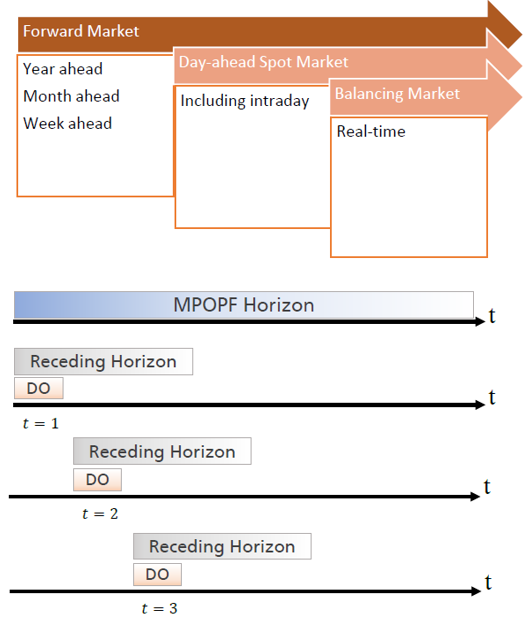
\includegraphics[scale=0.39]{Figures/ReceedingHorizon.png}
        \end{backgroundblock}}
\end{block}}
\visible<3-> {\begin{block}{Disadvantage of MultiPeriod ACOPF}
The problem grows very large as the number of time-steps is increased, which may lead to an intractable solution. 
\end{block}}
\end{frame}
%%%%%%%%%%%%%%%%%%%%%%%%%%%%%%%%%%%
%%%%%%%%%%%%%%%%%%%%%%%%%%%%%%%%%%%%
%%%%%%%%%%%%%%%%%%%%%%%%%%%%%%%%%%%
%%%%%%%%%%%%%%%%%%%%%%%%%%%%%%%%%
\begin{frame}{MultiPeriod ACOPF-problem formulation}

\begin{center}
\begin{tabular}{|l l|} 
\hline
Objective Function&$\min_{\mathbf{X}} F(\mathbf{X})$\\  
\rowcolor{Gray}
\begin{tabular}[l]{@{}l@{}}Equality Constraints\\ (Balance)\\ Power Flow \end{tabular}  &$\textrm{s.t. } G(\mathbf{X})= \begin{colorbmatrix}
   \widetilde{G}(\mathbf{X}) \
   \overline{G}(\mathbf{X}) \
   \overline{G}^s(\mathbf{X})
\end{colorbmatrix}^\top=0  \in   \mathbb{R}^{N_{g} \times 1}$\\
  
\begin{tabular}[l]{@{}l@{}}Inequality constraints\\ (line and transformer)\\ Operational Constraints \end{tabular}  & $H(\mathbf{X})=\begin{colorbmatrix}
   \widetilde{H}(\mathbf{X}) \quad
   \overline{H}(\mathbf{X})
\end{colorbmatrix}^\top\leq 0  \in   \mathbb{R}^{N_{h} \times 1} $\\
\rowcolor{Gray}
Vectors of Constraints&{\tiny \begin{tabular}[l]{@{}l@{}}$
   \widetilde{\mathbf{G}}(\mathbf{X})=
\begin{colorbmatrix}
    \widetilde{\mathbf{g}}(\mathbf{x}_{1}) \
    \widetilde{\mathbf{g}}(\mathbf{x}_{2}) \
    \dots \
    \widetilde{\mathbf{g}}(\mathbf{x}_{T}) 
\end{colorbmatrix}^\top$\\ $ 
   \overline{\mathbf{G}}(\mathbf{X})=
\begin{colorbmatrix}
    \overline{\mathbf{g}}(\mathbf{x}_{1}) \
    \overline{\mathbf{g}}(\mathbf{x}_{2}) \
    \dots \
    \overline{\mathbf{g}}(\mathbf{x}_{T}) \
\end{colorbmatrix}^\top $\\ $
  \overline{\mathbf{G}}^s(\mathbf{X})=
\begin{colorbmatrix}
    \overline{\mathbf{g}}^s(\boldsymbol{\tau}_1) \
    \overline{\mathbf{g}}^s(\boldsymbol{\tau}_2) \
    \dots \
    \overline{\mathbf{g}}^s(\boldsymbol{\tau}_T) 
\end{colorbmatrix}^\top  $\\ $
   \widetilde{\mathbf{H}}(\mathbf{X})=
\begin{colorbmatrix}
    \widetilde{\mathbf{h}}(\mathbf{x}_{1}) \
    \widetilde{\mathbf{h}}(\mathbf{x}_{2}) \
    \dots \
    \widetilde{\mathbf{h}}(\mathbf{x}_{T}) 
\end{colorbmatrix}^\top$\\ $
  \overline{\mathbf{H}}(\mathbf{X})= 
\begin{colorbmatrix}
    \overline{\mathbf{h}}(\mathbf{x}_{1}) \
    \overline{\mathbf{h}}(\mathbf{x}_{2}) \
    \dots \
    \overline{\mathbf{h}}(\mathbf{x}_{T}) 
\end{colorbmatrix}^\top $\end{tabular}  
}\\  
\hline
\end{tabular}
\end{center}



\end{frame}
%%%%%%%%%%%%%%%%%%%%%%%%%%%%%%%%%
%%%%%%%%%%%%%%%%%%%%%%%%%%%%%%%%%%%
%%%%%%%%%%%%%%%%%%%%%%%%%%%%%%%%%%%%
%%%%%%%%%%%%%%%%%%%%%%%%%%%%%%%%%%%
%%%%%%%%%%%%%%%%%%%%%%%%%%%%%%%%%
\section{Solution Method}
\begin{frame}{Nonlinear Programming (NLP)}
\begin{block}{How do we solve Optimal Power Flow?}
\begin{enumerate}[I.]
\item<1-> Interior Point Method
\item<2-> Gradient Decent Method
\item<3-> Heuristic Methods 
\end{enumerate}
\end{block}
\onslide<4>{\begin{alertblock}
{Interior Point Method}
The focus of this study is the interior point method solution
\end{alertblock}}
\end{frame}
%%%%%%%%%%%%%%%%%%%%%%%%%%%%%%%%%
%%%%%%%%%%%%%%%%%%%%%%%%%%%%%%%%%%%
%%%%%%%%%%%%%%%%%%%%%%%%%%%%%%%%%%%%
%%%%%%%%%%%%%%%%%%%%%%%%%%%%%%%%%%%
%%%%%%%%%%%%%%%%%%%%%%%%%%%%%%%%%

\begin{frame}

\begin{center}
\begin{tabular}{|l|} 
\hline
\rowcolor{yellow}
Step(1): Applying Slack variables and the barrier term: \\
\rowcolor{Gray}

$\min_{\mathbf{X}} \bigg[F(\mathbf{X})-\gamma\sum_{i=1}^{N_h}{ln(z_{i})}\bigg]$\\ \rowcolor{Gray}

 $\textrm{s.t. }  \mathbf{G}(\mathbf{X})=0$\\ \rowcolor{Gray}

$\mathbf{H}(\mathbf{X})+\mathbf{Z}=0$\\ \rowcolor{Gray}

 $\mathbf{Z}\geq 0$\\
\hline
slack variables "Z" convert inequality constraints to equality constraints.\\
\hline
\end{tabular}
\end{center}

\end{frame}

%%%%%%%%%%%%%%%%%%%%%%%%%%%%%%%%%
%%%%%%%%%%%%%%%%%%%%%%%%%%%%%%%%%%%
%%%%%%%%%%%%%%%%%%%%%%%%%%%%%%%%%%%%
%%%%%%%%%%%%%%%%%%%%%%%%%%%%%%%%%%%
%%%%%%%%%%%%%%%%%%%%%%%%%%%%%%%%%


\begin{frame}
\begin{center}
\begin{tabular}{|l l|} 
\hline
\rowcolor{cyan} \multicolumn{2}{|l|}{Step (2): Calculate and form the Lagrangian of Barrier subproblem} \\
\rowcolor{Gray} \multicolumn{2}{|l|}{ $\boldsymbol{\mathcal{L}}^{\gamma}(\mathbf{X},\mathbf{Z},\boldsymbol{\lambda},\boldsymbol{\mu})=f(\mathbf{X})+\boldsymbol{\lambda}^\top \mathbf{G}(\mathbf{X})
+\boldsymbol{\mu}^\top(\mathbf{H}(\mathbf{X})+\mathbf{Z})-\gamma \sum_{i=1}^{N_g}{ln(z_{i})}$}\\
\hline
\multicolumn{2}{l}{}\\
\multicolumn{2}{l}{}\\
\hline
\rowcolor{magenta}
\multicolumn{2}{|l|}{Step (3): Calculate the KKT\footnote{Karush–Kuhn–Tucker conditions} of the Lagrangian}\\
\rowcolor{Gray}
\begin{tabular}[l]{@{}l@{}}Step (3)\\$KKT_X$  \end{tabular} &$\boldsymbol{\mathcal{L}}_{\mathbf{X}}^{\gamma}(\mathbf{X},\mathbf{Z},\boldsymbol{\lambda},\boldsymbol{\mu})=f_{\mathbf{X}}+\boldsymbol{\lambda}^\top \mathbf{G}_{\mathbf{X}}+\boldsymbol{\mu}^\top \mathbf{H}_{\mathbf{X}}=0$\\
\rowcolor{Gray}
\begin{tabular}[l]{@{}l@{}}Step (3)\\$KKT_Z$  \end{tabular}&$\boldsymbol{\mathcal{L}}_{\mathbf{Z}}^{\gamma}(\mathbf{X},\mathbf{Z},\boldsymbol{\lambda},\boldsymbol{\mu})=\boldsymbol{\mu}^\top - \gamma \mathbf{e}^\top\mathbf{diag}(\mathbf{Z})^{-1}=0$\\  
\rowcolor{Gray}
\begin{tabular}[l]{@{}l@{}}Step (3)\\$KKT_\lambda$   \end{tabular}  &$\boldsymbol{\mathcal{L}}_{\boldsymbol{\lambda}}^{\gamma}(\mathbf{X},\mathbf{Z},\boldsymbol{\lambda},\boldsymbol{\mu})=\mathbf{G}^\top (\mathbf{X})=0$
\\
  \rowcolor{Gray}
\begin{tabular}[l]{@{}l@{}}Step (3)\\$KKT_\mu$   \end{tabular}    & $
\boldsymbol{\mathcal{L}}_{\boldsymbol{\mu}}^{\gamma}(\mathbf{X},\mathbf{Z},\boldsymbol{\lambda},\boldsymbol{\mu})=\mathbf{H}^\top(\mathbf{X})+\mathbf{Z}^\top=0$\\ 
\hline
\end{tabular}
\end{center}


\end{frame}
%%%%%%%%%%%%%%%%%%%%%%%%%%%%%%%%%
%%%%%%%%%%%%%%%%%%%%%%%%%%%%%%%%%%%
%%%%%%%%%%%%%%%%%%%%%%%%%%%%%%%%%%%%
%%%%%%%%%%%%%%%%%%%%%%%%%%%%%%%%%%%
%%%%%%%%%%%%%%%%%%%%%%%%%%%%%%%%%


\begin{frame}

\begin{center}
\begin{tabular}{|l l|} 
\hline
Nonlinear Algebraic Equations&$\boldsymbol{\Omega}(\mathbf{X},\mathbf{Z},\boldsymbol{\lambda},\boldsymbol{\mu})
=\begin{bmatrix}
    f_{\mathbf{X}}+\boldsymbol{\lambda}^\top \mathbf{G}_{\mathbf{X}}+\boldsymbol{\mu}^\top \mathbf{H}_{\mathbf{X}} \\
   \mathbf{diag}(\mathbf{Z})\boldsymbol{\mu}^\top - \gamma \mathbf{e}^\top\\
    \mathbf{G}^\top (\mathbf{X})\\
    \mathbf{H}^\top(\mathbf{X})+\mathbf{Z}^\top
\end{bmatrix}=0$\\

$S.t.$&$\quad \mathbf{Z} > 0$\\

&$\quad \boldsymbol{\mu} > 0$\\  
\hline
\multicolumn{2}{l}{}\\
\hline
\rowcolor{green}
\multicolumn{2}{|l|}{Step (4): Apply Newton Raphson Method}\\
\rowcolor{Gray}
\multicolumn{2}{|l|}{ \quad $[\boldsymbol{\Omega}_\mathbf{X} \ \boldsymbol{\Omega}_\mathbf{Z} \ \boldsymbol{\Omega}_{\boldsymbol{\lambda}} \ \boldsymbol{\Omega}_{\boldsymbol{\mu}}]^k{[\Delta \mathbf{X} \ \Delta \mathbf{Z} \ \Delta \boldsymbol{\lambda} \ \Delta \boldsymbol{\mu}]^\top}^k=-\boldsymbol{\Omega}(\mathbf{X},\mathbf{Z},\boldsymbol{\lambda},\boldsymbol{\mu})^k$}\\
\hline
\end{tabular}
\end{center}

\end{frame}

%%%%%%%%%%%%%%%%%%%%%%%%%%%%%%%%%
%%%%%%%%%%%%%%%%%%%%%%%%%%%%%%%%%%%
%%%%%%%%%%%%%%%%%%%%%%%%%%%%%%%%%%%%
%%%%%%%%%%%%%%%%%%%%%%%%%%%%%%%%%%%
%%%%%%%%%%%%%%%%%%%%%%%%%%%%%%%%%
\begin{frame}
\begin{center}
\begin{tabular}{|l l|} 
\hline 
\begin{tabular}[l]{@{}l@{}}Step (5): \\{Inverse Jacobian} \\ of Newton Raphson  \end{tabular} \cellcolor{red} & \cellcolor{Gray}${\textcolor{red}{\begin{colorbmatrix}
    \mathbf{M}&  \mathbf{G}_{\mathbf{X}}^\top\\
    \mathbf{G}_{\mathbf{X}} & 0\\
\end{colorbmatrix}}}^k
{\begin{colorbmatrix}
    \Delta \mathbf{X}\\
   \Delta\boldsymbol{\lambda}
\end{colorbmatrix}}^k=
{\begin{colorbmatrix}
    -\mathbf{N}\\
   -\mathbf{G}(\mathbf{X})
\end{colorbmatrix}}^k $\\
\hline
\end{tabular}
\end{center}
$\mathbf{M} \in \mathbb{R}^{N_x \times N_x}$ and $\mathbf{N} \in \mathbb{R}^{N_x \times 1}$ are defined as:


\begin{center}
\begin{tabular}{|l l|} 
\hline
&$ \mathbf{M}=\boldsymbol{\mathcal{L}}_{\mathbf{X}\mathbf{X}}^{\gamma}+\mathbf{H}_{\mathbf{X}}^\top\mathbf{diag}(\mathbf{Z})^{-1}\mathbf{diag}(\boldsymbol{\mu}) \mathbf{H}_{\mathbf{X}}$\\

&$\mathbf{N}=f_{\mathbf{X}}^\top+\mathbf{G}_{\mathbf{X}}^\top\boldsymbol{\lambda}+\mathbf{H}_{\mathbf{X}}^\top\boldsymbol{\mu} +\mathbf{H}_{\mathbf{X}}^\top\mathbf{diag}(\mathbf{Z})^{-1}(\gamma \mathbf{e} +\mathbf{diag}(\boldsymbol{\mu})\mathbf{H}(\mathbf{X}))$\\

&$\boldsymbol{\mathcal{L}}_{\mathbf{X}\mathbf{X}}^{\gamma} = f_{\mathbf{XX}}+\mathbf{G}_{\mathbf{XX}}(\boldsymbol{\lambda})+\mathbf{H}_{\mathbf{XX}}(\boldsymbol{\mu})$\\
\hline
\end{tabular}
\end{center}

\end{frame}
%%%%%%%%%%%%%%%%%%%%%%%%%%%%%%%%%
%%%%%%%%%%%%%%%%%%%%%%%%%%%%%%%%%%%
%%%%%%%%%%%%%%%%%%%%%%%%%%%%%%%%%%%%
%%%%%%%%%%%%%%%%%%%%%%%%%%%%%%%%%%%
%%%%%%%%%%%%%%%%%%%%%%%%%%%%%%%%%
\begin{frame}{Iterations}
\vskip -1.5cm
\begin{block}{Successive iterations in Interior Point Method}
\begin{enumerate}[i.]
\item<1-> \textcolor{gray}{\textbf{Function Evaluations}} \only<1> {calculation of $\mathbf{G}_{\mathbf{X}}=\frac{\partial \mathbf{G}}{\partial \mathbf{X}}$, $\mathbf{H}_{\mathbf{X}}=\frac{\partial \mathbf{H}}{\partial \mathbf{X}}$, $F_{\mathbf{X}}=\frac{\partial F}{\partial \mathbf{X}}$, $\mathbf{G}_{\mathbf{X}\mathbf{X}}=\frac{\partial}{\partial \mathbf{X}}(\mathbf{G}_\mathbf{X}^\top \boldsymbol{\lambda})$, $\mathbf{H}_{\mathbf{X}\mathbf{X}}=\frac{\partial}{\partial \mathbf{X}}(\mathbf{H}_\mathbf{X}^\top \boldsymbol{\lambda})$, $F_{\mathbf{X}\mathbf{X}}=\frac{\partial}{\partial \mathbf{X}}({F}_\mathbf{X}^\top)$ in order to form coefficient matrix and right hand side of ${\begin{colorbmatrix}
    \mathbf{M}&  \mathbf{G}_{\mathbf{X}}^\top\\
    \mathbf{G}_{\mathbf{X}} & 0\\
\end{colorbmatrix}}^k
{\begin{colorbmatrix}
    \Delta \mathbf{X}\\
   \Delta\boldsymbol{\lambda}
\end{colorbmatrix}}^k=
{\begin{colorbmatrix}
    -\mathbf{N}\\
   -\mathbf{G}(\mathbf{X})
\end{colorbmatrix}}^k $}
\item<2-> \textcolor{mine1}{\textbf{Linear Algebraic Solver}} \only<2>{Calculate the Inverse ${\begin{colorbmatrix}
    \mathbf{M}&  \mathbf{G}_{\mathbf{X}}^\top\\
    \mathbf{G}_{\mathbf{X}} & 0\\
\end{colorbmatrix}}^k$ in ${\begin{colorbmatrix}
    \mathbf{M}&  \mathbf{G}_{\mathbf{X}}^\top\\
    \mathbf{G}_{\mathbf{X}} & 0\\
\end{colorbmatrix}}^k
{\begin{colorbmatrix}
    \Delta \mathbf{X}\\
   \Delta\boldsymbol{\lambda}
\end{colorbmatrix}}^k=
{\begin{colorbmatrix}
    -\mathbf{N}\\
   -\mathbf{G}(\mathbf{X})
\end{colorbmatrix}}^k $} 
\item<3-> \textcolor{mine2}{\textbf{Miscellaneous}} \only<3>{ Computational time for other components of IP such as step control and step update: $X^{k+1}=X^k+\Delta X $}
\item<4-> Bottleneck of IP:  
\only<4>{ 
\begin{backgroundblock}{50mm}{50mm}
        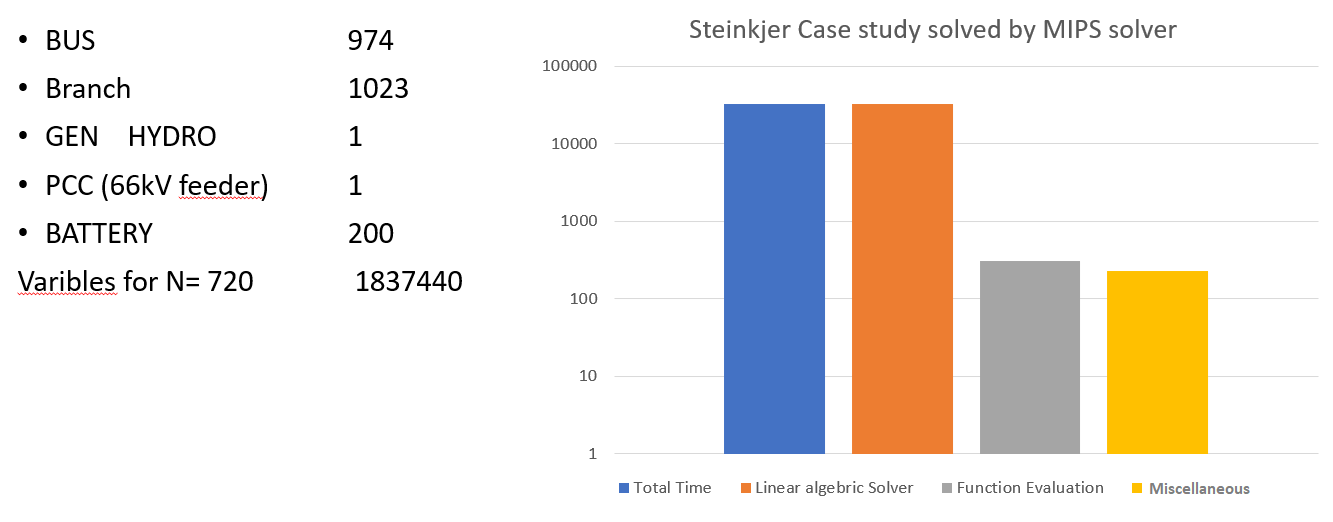
\includegraphics[width=3.5 in , height=1.5 in]{Figures/IPbottleneck.png}
        \end{backgroundblock}}
\end{enumerate}
\end{block}
\end{frame}





\section{Speed-up the solution proposal}
\subsection{Reordering}
\begin{frame}
\begin{figure}[!htbp]
\centering
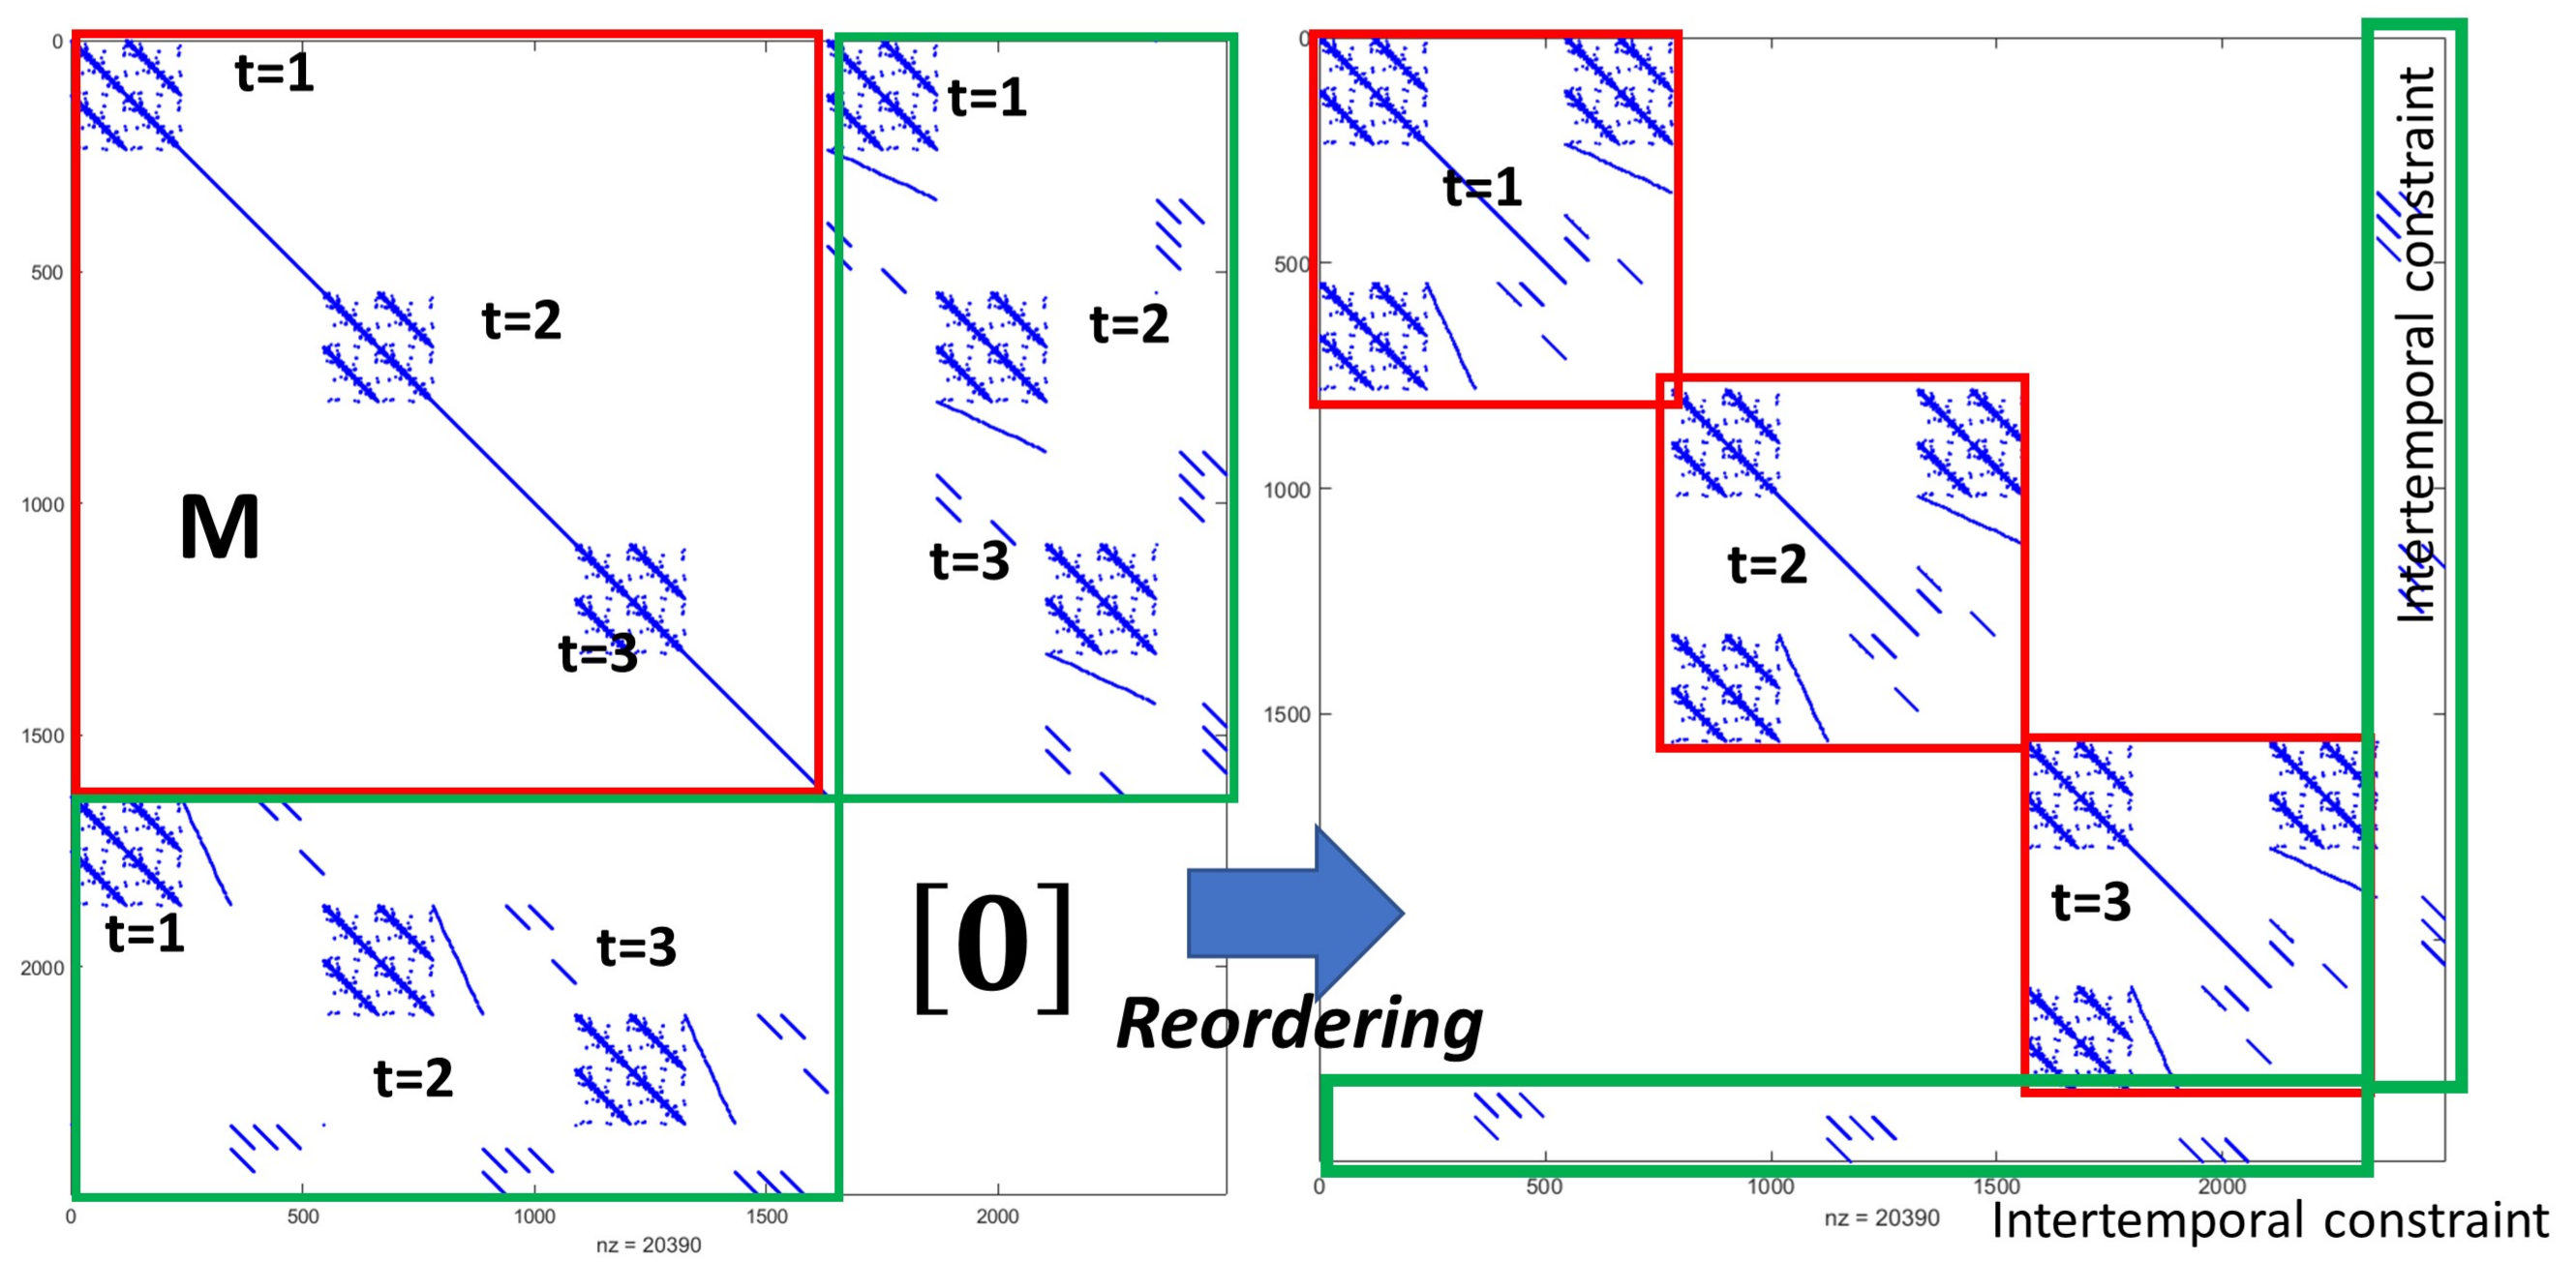
\includegraphics[width=3.4 in , height=1.7 in]{Figures/reorder.png}
% where an .eps filename suffix will be assumed under latex,
% and a .pdf suffix will be assumed for pdflatex; or what has been declared
% via \DeclareGraphicsExtensions.
\caption{Structure of Jacobian of the Newton-Raphson's algorithm before and after reordering.}
\label{fig:1}\vspace*{-0.4cm}
\end{figure} 
\begin{alertblock}{Jacobian of Newton-Raphson}
\centering
{\tiny
${\textcolor{red}{\begin{colorbmatrix}
    \mathbf{M}&  \mathbf{G}_{\mathbf{X}}^\top\\
    \mathbf{G}_{\mathbf{X}} & 0\\
\end{colorbmatrix}}}
{\begin{colorbmatrix}
    \Delta \mathbf{X}\\
   \Delta\boldsymbol{\lambda}
\end{colorbmatrix}}=
{\begin{colorbmatrix}
    -\mathbf{N}\\
   -\mathbf{G}(\mathbf{X})
\end{colorbmatrix}} $\\
The solution is published in Papers I and II of this thesis.}
\end{alertblock}
 \end{frame}
%%%%%%%%%%%%%%%%%%%%%%%%%%%%%%%%%
%%%%%%%%%%%%%%%%%%%%%%%%%%%%%%%%%%%
%%%%%%%%%%%%%%%%%%%%%%%%%%%%%%%%%%%%
%%%%%%%%%%%%%%%%%%%%%%%%%%%%%%%%%%%
%%%%%%%%%%%%%%%%%%%%%%%%%%%%%%%%%
\section{Results}
\subsection{Schur-Complement}
\begin{frame}
\begin{figure}[!htbp]
\centering
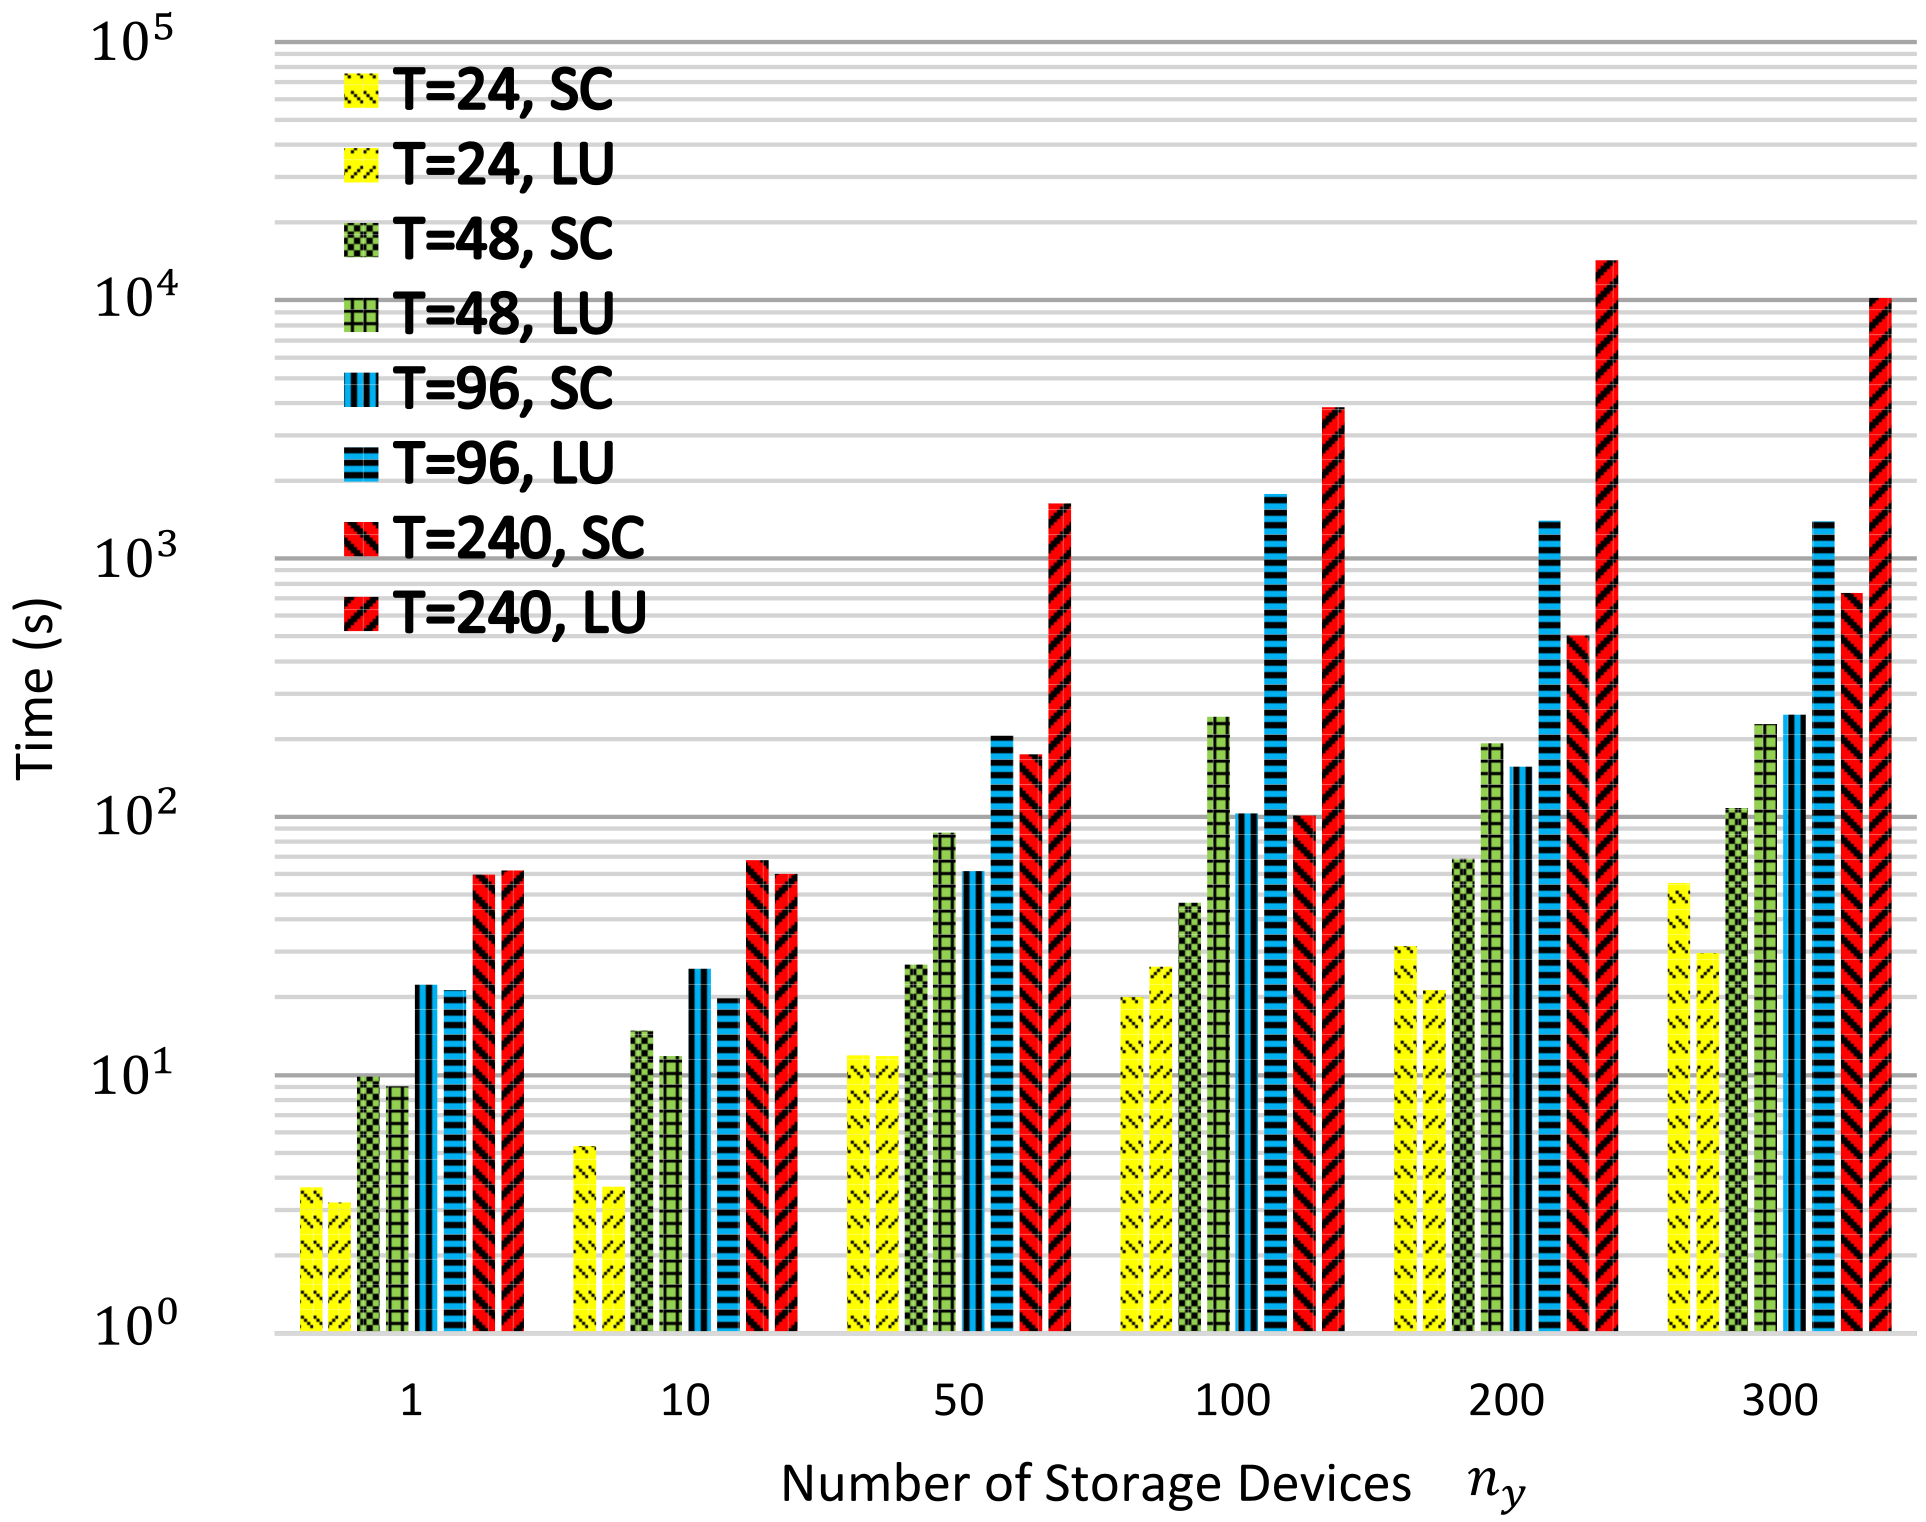
\includegraphics[width=3.0 in , height=2.5 in]{Figures/SCLU118Bus.png}
\caption{Total time ($\mathrm{TotalTime= No_{\cdot} of \ Iter_{\cdot} \times TimePerIter}$) for solution of the linear KKT systems, Case: IEEE 118.}
\label{118bus}
\end{figure}
\end{frame}

%%%%%%%%%%%%%%%%%%%%%%%%%%%%%%%%%
%%%%%%%%%%%%%%%%%%%%%%%%%%%%%%%%%%%
%%%%%%%%%%%%%%%%%%%%%%%%%%%%%%%%%%%%
%%%%%%%%%%%%%%%%%%%%%%%%%%%%%%%%%%%
%%%%%%%%%%%%%%%%%%%%%%%%%%%%%%%%%


\subsection{Analytical Derivatives}

\begin{frame}{Analytical Derivatives}
\vskip -0.6cm
\begin{table}
\tiny
\begin{center}
 \caption{Total time ($\mathrm{TotalTime= No_{\cdot} of \ Iter_{\cdot} \times TimePerIter}$) elapsed to calculate: 1) Analytical (hand-coded) derivatives, and 2) Numerical derivatives }
\label{tab:numericVSanalytic}
\begin{threeparttable}
\begin{tabularx}{\textwidth}{m s s s s c s s s c m }
\toprule
&&&&   \multicolumn{3}{c}{Analytical}&&\multicolumn{3}{c}{Numerical} \\
\cmidrule{5-7}  \cmidrule{9-11} 
Case     & $T$&$n_y$ &iter & ${F}_\mathbf{X}$(s)&$\mathbf{G}_\mathbf{X}$+ $\mathbf{H}_\mathbf{X}$(s)&$\boldsymbol{\mathcal{L}}_{\mathbf{X}\mathbf{X}}^{\gamma}$(s)& &${F}_\mathbf{X}$(s)&$\mathbf{G}_\mathbf{X}$+ $\mathbf{H}_\mathbf{X}$(s)&$\boldsymbol{\mathcal{L}}_{\mathbf{X}\mathbf{X}}^{\gamma}$(s) \\ 
\midrule
Case9     &2 &5&13& 0.03 & 0.13 & 0.14 & &0.43 & 0.98 &140.07\\ 
Case9     &10&5&23& 0.08  & 0.36 & 0.37 & &11.32 & 30.62  & 22815.29\\ 
IEEE30    &2&5&12 & 0.04 & 0.25 & 0.18     &   & 1.01  & 2.16  & 682.70\\ 
IEEE30    &10&5&16& 0.05 & 0.24 & 0.25 && 16.73 & 49.12  & 79712.78\\ 
IEEE118   &2&5&22 & 0.04 & 0.19 & 0.20   & &7.41 & 18.07 & 24557.09\\ 
IEEE118   &10&5&37&  0.09 & 0.62 & 0.82   & & 158.21\tnote{1}  & 572.09 \tnote{1} & 4599735\tnote{1} \\ 
PEGASE1354&2 &5&23& 0.05 & 0.61 & 0.78    & &85.54\tnote{1}  & 496.18 \tnote{1} & 7185888 \tnote{1}  \\ 
PEGASE1354&10&5&33& 0.10 & 3.77 & 5.15  & & 588.06\tnote{1}  & 3530  \tnote{1} & 51550941\tnote{1}  \\ 
\bottomrule
\end{tabularx}
\begin{tablenotes}
\item[1] {Estimated total time: The time elapsed for one iteration multiplied to the iteration that would take to converge}
\end{tablenotes}
\end{threeparttable}
\end{center}
\end{table}
\begin{alertblock}{Test Cases}
Test cases of Case9, IEEE30, IEEE118, and PEGASE1354 are part of open source MATPOWER library.
\end{alertblock}
\end{frame}



\begin{frame}
\begin{figure}[!htbp]
\centering
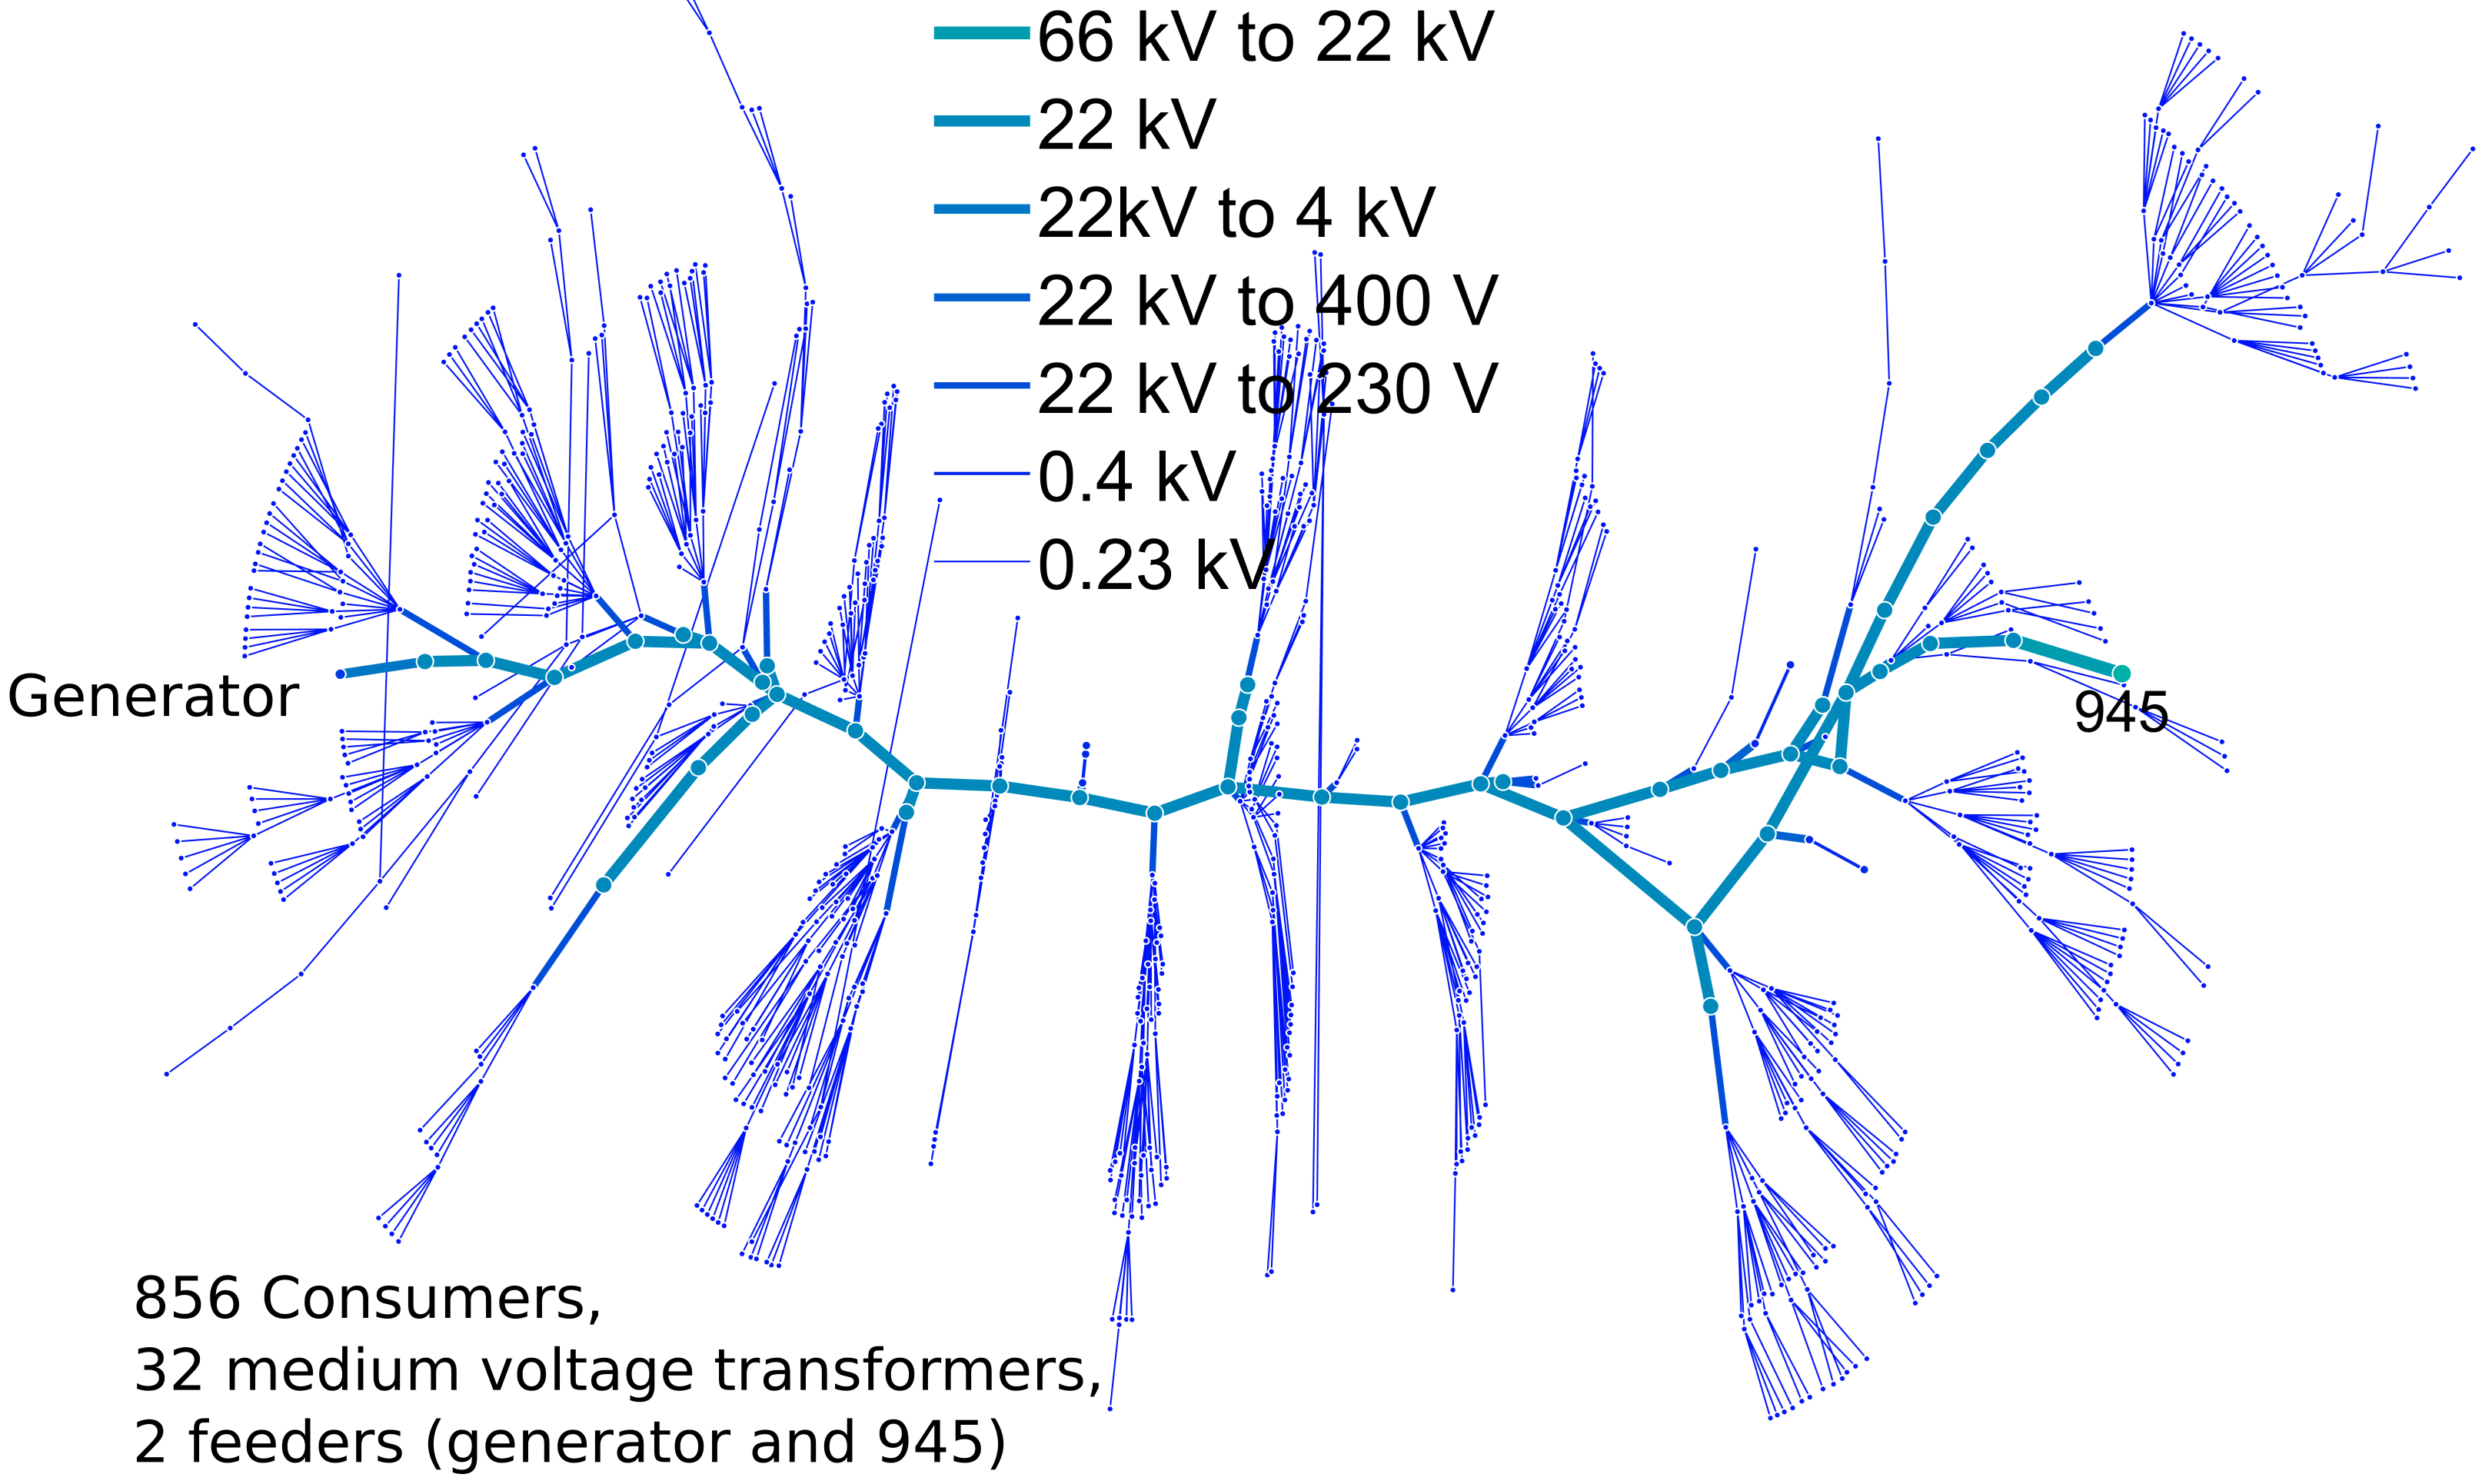
\includegraphics[width=4 in , height=2.5 in]{Figures/DistributionGridmodified.png}
\caption{\vspace*{-0.4cm} Local distribution grid located in Norway with 856 costumers}
\label{Norwegian1}
\end{figure}
\end{frame}

\begin{frame}{Norwegian grid with 856 consumers}

{\tiny
\begin{table}
\caption{[a) total energy production, b) active system loss, and c) system cost] in three different operational modes.}
\begin{tabular}{l c c c c c c} 
\toprule \rowcolor{Gray}
 {\scriptsize Method} & \begin{tabular}[l]{@{}l@{}}Daily \\Energy \\ Consumption\\(MWh)  \end{tabular}& \begin{tabular}[l]{@{}l@{}}LOSS \\(MWh) \end{tabular}&
 \begin{tabular}[l]{@{}l@{}}System \\Cost\\ (kNOK)\end{tabular} &  \begin{tabular}[l]{@{}l@{}}Daily\\Saving\\ (NOK)--(\%) \end{tabular} &  \begin{tabular}[l]{@{}l@{}}Yearly \\Saving\\ (kNOK)--(\%) \end{tabular}  & \begin{tabular}[l]{@{}l@{}}Max \\EV\\ Hosting\\Capacity \end{tabular}\\  
\midrule \midrule
\begin{tabular}[l]{@{}l@{}}Dumb \\Charging \end{tabular}&118.64 & 9.0 & 76  & -- & -- &220 EV (20\%) \\
\midrule \rowcolor{Gray}
\begin{tabular}[l]{@{}l@{}}MPOPF \\without\\operational \\limits \end{tabular} & 118.74&8.6 & 74 & 1,846 -- 2.4 \%  & 674& 400 EV (36\%) \\
\midrule
\begin{tabular}[l]{@{}l@{}}MPOPF \\with\\operational \\limits \end{tabular}&118.74&8.6 & 75 & 1,184 -- 1.6 \% & 432& 1113 EV (100\%) \\
\bottomrule
\end{tabular}
\end{table}
}
\end{frame}

\section{Response to RQs}
\begin{frame}{Brief Response to RQs}
\begin{enumerate}[label=\textbf{RQ {\arabic*}.},ref=RQ {\arabic*}.]
\item<1> \label{int:RQ1} With only ``passive charging'', the deployment of EVs will be limited by grid constraints. Can ``smart-charging'' overcome this problem?\\
\only<1> { \begin{block}{Answer to RQ1. [Papers III and V]}
Yes, it can. Simulation results on real data show that a centralised EV charging scheduling with consideration of operational constraints could be a solution for overloading of transformer and lines plus voltage constraints.
\end{block} }
\item<2> \label{int:RQ2} How many additional EVs can be served by fast-charging points with a ``smart-charging'' regime compared to ``passive charging''? 
\begin{enumerate}[label=\textbf{C {\arabic*}.},ref=C {\arabic*}.]
\item<2> \label{int:con1}  Without any reinforcements of the grid. 
\item<2> \label{int:con2} Without any reduction in driving range.
\end{enumerate}\only<2> { \begin{block}{Answer to RQ2. [Papers III and VIII]} 100\% EV share of EV could be charged with no issue, while maximum 20\% EV share could be charged with dumb charging strategy.\end{block}}
\item<3-> \vskip -0.1cm \label{int:RQ3} How much grid reinforcements is needed with smart vs passive-charging to fulfill increasing targets for an EV fleet as a replacement for gasoline and diesel cars?
\only<3> {\vskip -0.1cm \begin{block}{Answer to RQ3. [Papers III, V and VII]}
No grid reinforcement is needed with smart strategy. Research should be conducted to clear how much grid reinforcement is required for dumb charging strategy.
\end{block}}

\item<4-> \label{int:RQ4} Could integration of PV mitigate the impact of increasing EV penetration on the distribution grid?
\only<4> { \vskip -0.2cm \begin{block}{Answer to RQ4. [Paper V]}
Yes. It can.
\end{block}}
\end{enumerate}
\end{frame}
\section{Conclusion}
\begin{frame}{Conclusion}
\onslide<1-> \begin{block}{P 1.}In this thesis, a new toolbox is developed for large integration of EV and stationary ESS.\end{block}
\onslide<2-> \begin{block}{P 2.} A route to high performance power flow solver is taken. \end{block}
\onslide<3-> \begin{block}{P 3.} Real data w.r.t local distribution grid and EV charging are taken and tested to confirm and withhold hypothesis. \end{block}
\end{frame}


\end{document}
